% Chapter Template

\chapter{The KOTO Experiment} % Main chapter title

\label{Chapter3} % Change X to a consecutive number; for referencing this chapter elsewhere, use \ref{ChapterX}

% outline
%----------------------------------------------------------------------------
% 3-1 : Basic strategy
% 3-2 : Accelerator
% 3-3 : Detector

KOTO is the first dedicated experiment to search for the $K_L^0 \to \pi^0 \nu \overline{\nu}$ decay. Because the SM prediction for $\mathcal{BR}(K_L^0 \to \pi^0 \nu \bar{\nu})$ is $\mathcal{O}(10^{-11})$, the high-intensity $K_L^0$ beam is produced to reach the SM sensitivity within a reasonable time frame. Moreover, the KOTO detector is exclusively designed for the massive background suppression. With all these features, the KOTO experiment is able to explore the unprecedented sensitivities to the ${K_L^0 \to \pi^0 \nu \bar{\nu}}$ decay and even unfold the secret in CP violation.

%All these features are briefly introduced in this chapter.
%All these features are crucial for KOTO to explore unprecedented sensitivities to the $K_L^0 \to \pi^0 \nu \overline{\nu}$ decay and briefly introduced in this chapter. 
%With all these features, the KOTO experiment is able to explore unprecedented sensitivities to the $K_L^0 \to \pi^0 \nu \overline{\nu}$ decay.
%In this chapter, the basic strategy to search for the ${K_L^0 \to \pi^0 \nu \overline{\nu}}$ decay is first introduced. An overview of the accelerator to produce the $K_L^0$ beam and the KOTO detector is then presented. 

%----------------------------------------------------------------------------------------
%	SECTION 1: basic strategy
%----------------------------------------------------------------------------------------

\section{Basic Strategy of the KOTO experiment}
\label{sec:basic}

Figure~\ref{fig:schematic_KOTO} shows how KOTO searches for the ${K_L^0 \to \pi^0 \nu \overline{\nu}}$ decay. A bunch of protons first collides at the gold target and the secondary particles are guided to a beamline at $16^{\circ}$ \parencite{KL_beamline}. The KOTO detector is 21~m away from the target and hence most of the short-lived particles have already decayed. Furthermore, the photon absorber and the sweeping magnet are installed to wipe out photons and charged particles. The two collimaters are constructed to ensure the beam is pencil-like. The survivals that can enter the KOTO detector are dominated by the long-lived neutral particles: $K_L^0$, neutrons, and photons. In order to eliminate the neutrons scattered in the beamline, the beam profile monitor \parencite{BPM} is managed to explicitly align the collimators.

\index{collimator}

\begin{figure}[h]
\begin{center}
\captionsetup{width=.99\linewidth}
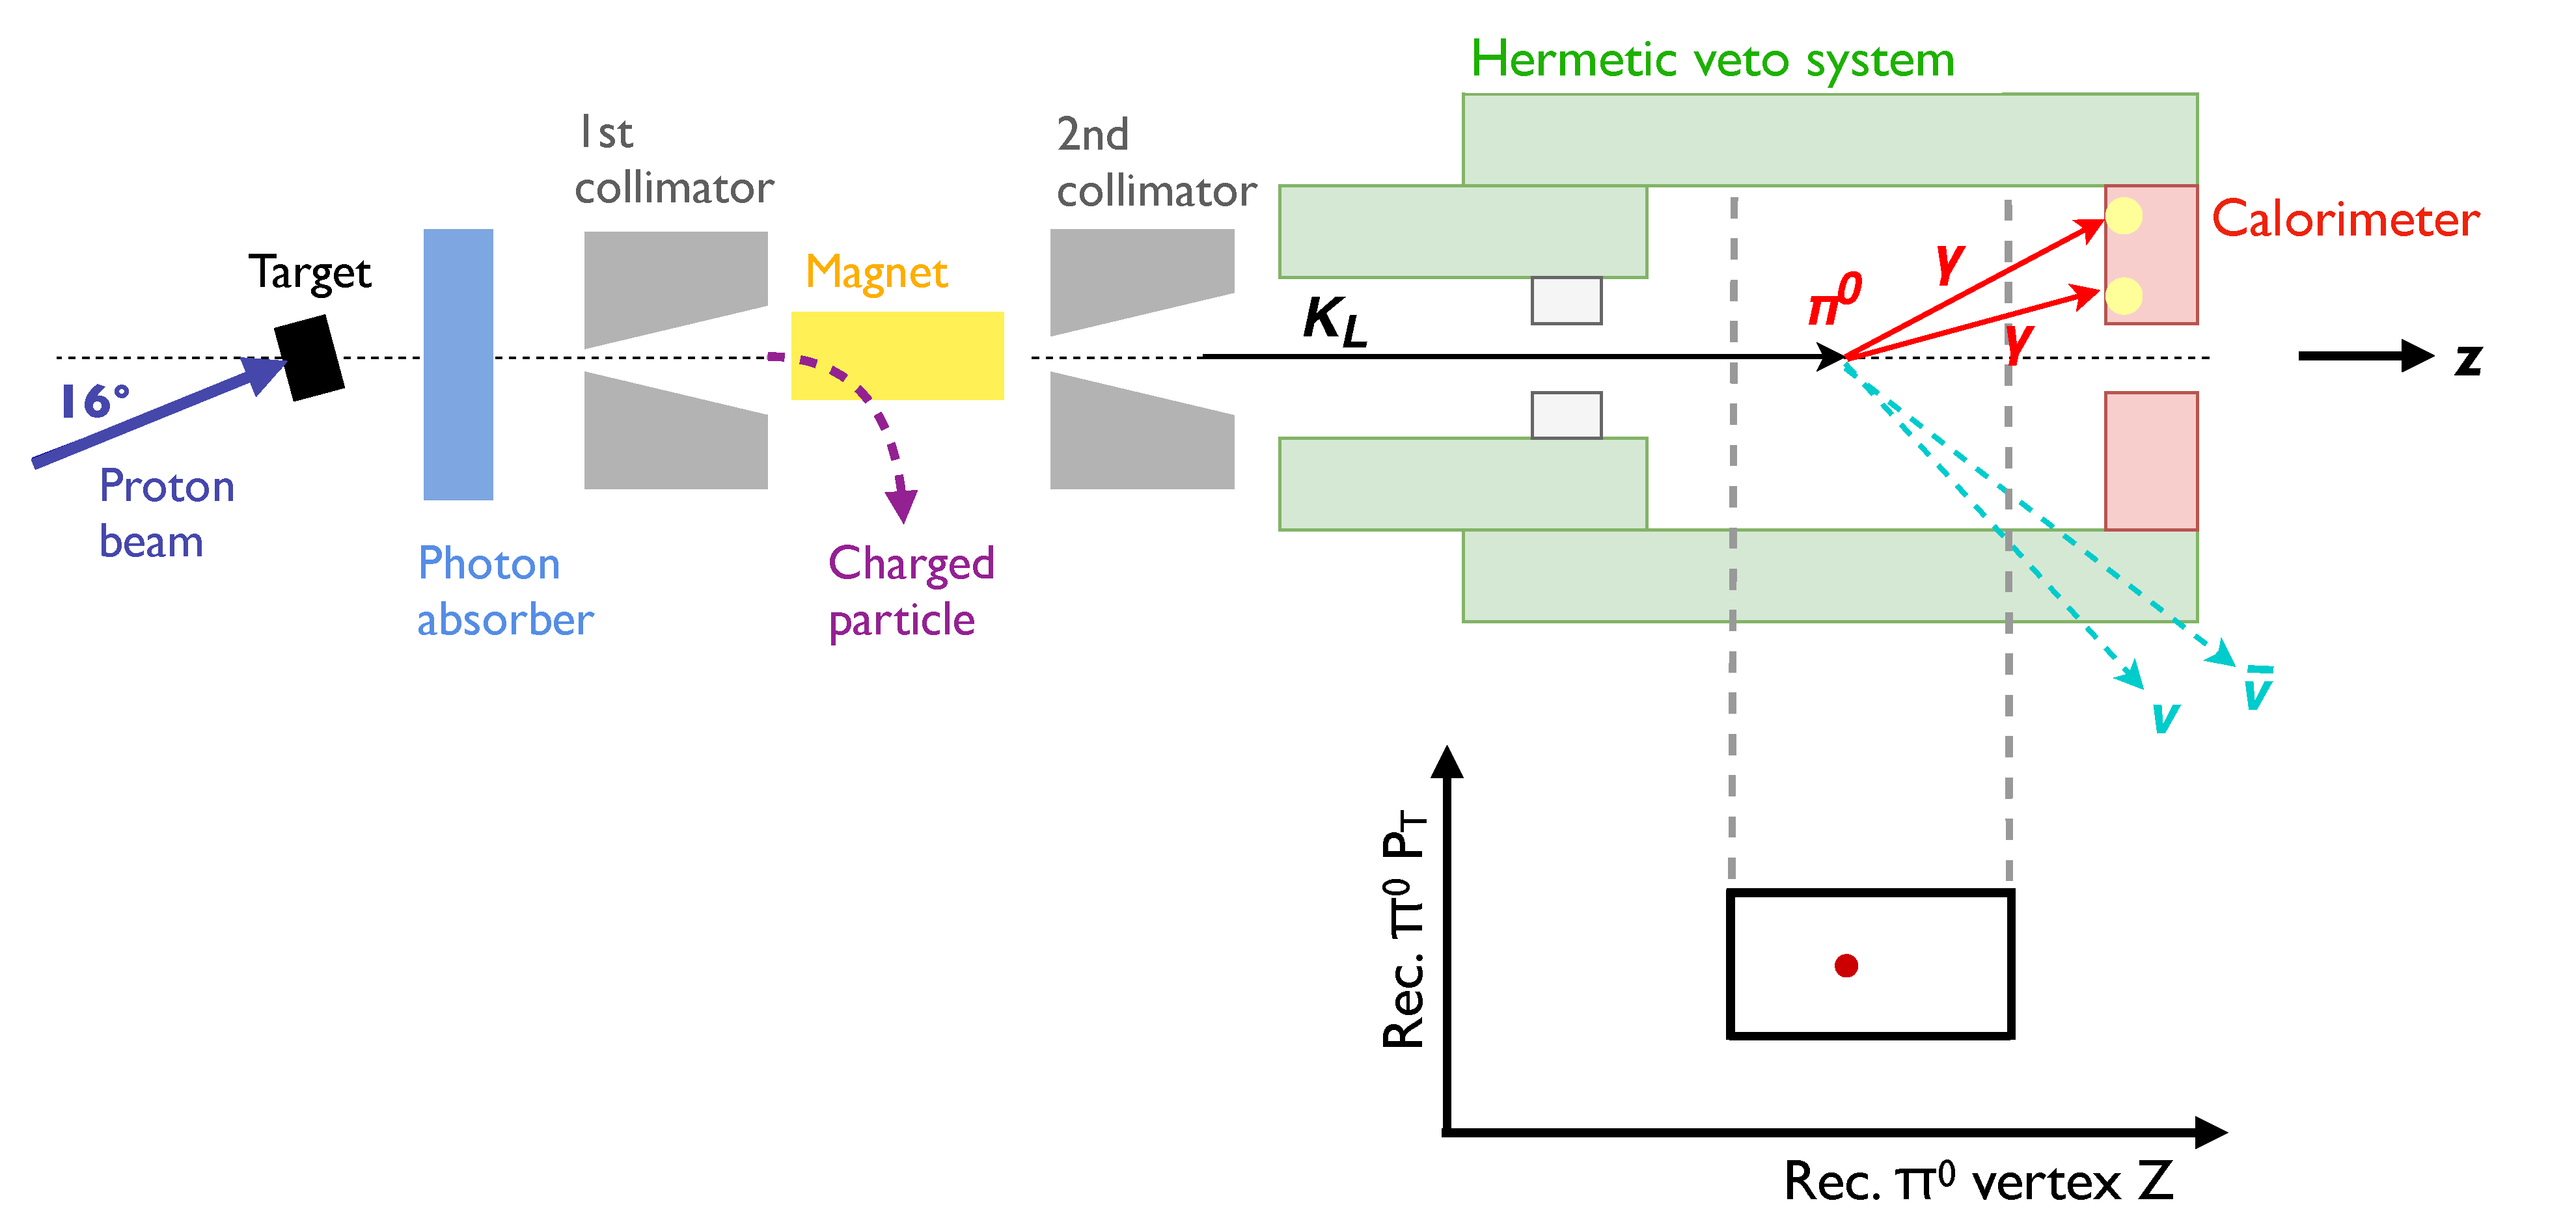
\includegraphics[width=0.99\textwidth]{Figures/Chapter3/schematic_ptz.pdf}
\caption{A schematic diagram of the search for $K_L^0 \to \pi^0 \nu \overline{\nu}$ at the KOTO experiment. }
\label{fig:schematic_KOTO}
\end{center}
\end{figure}

%%%%
% 3-1-1 signal identification

\subsection{Signal identification}

A reconstructable event requires exact two photons from a $\pi^0$ hitting the calorimeter, as shown in Figure \ref{fig:KOTO_signal_3D}. Based on four-momentum conservation, the opening angle ($\theta$) between two photons is calculated by %\mynobreakpar
%
\vspace{1em}
\begin{align}
\cos{\theta} = 1 - \frac{M_{\pi^0}^2}{2 E_1 E_2 },
\end{align}

\noindent 
where $E_1$ and $E_2$ are the two photon energies, and $M_\pi^0$ is the nominal $\pi^0$ mass. By assuming the $\pi^0$ decays at the center of the beam  (z-axis by convention), the $\pi^0$ vertex $Z$ ($Z_{vtx}$) can be obtained. Subsequently, the momenta of the two photons and the $\pi^0$ can be therefore calculated. Because neutrinos are invisible, the $\pi^0$ transverse momentum ($P_T$) is expected to be large.  

The signal box is defined on the reconstructed $(P_T - Z_{vtx})$ plane, as shown in the bottom part of Figure \ref{fig:schematic_KOTO}. Any event lies inside the signal box is treated as the "signal candidate". During the analysis, the side-band region is utilized to predict the distribution inside the signal region. Not until the data behavior is fully understood can the events in the signal region be accessed. This strategy, so-called "blind analysis", is adopted to dispel the prejudice against the signal candidates.

\begin{figure}[h]
\begin{center}
\captionsetup{width=.99\linewidth}
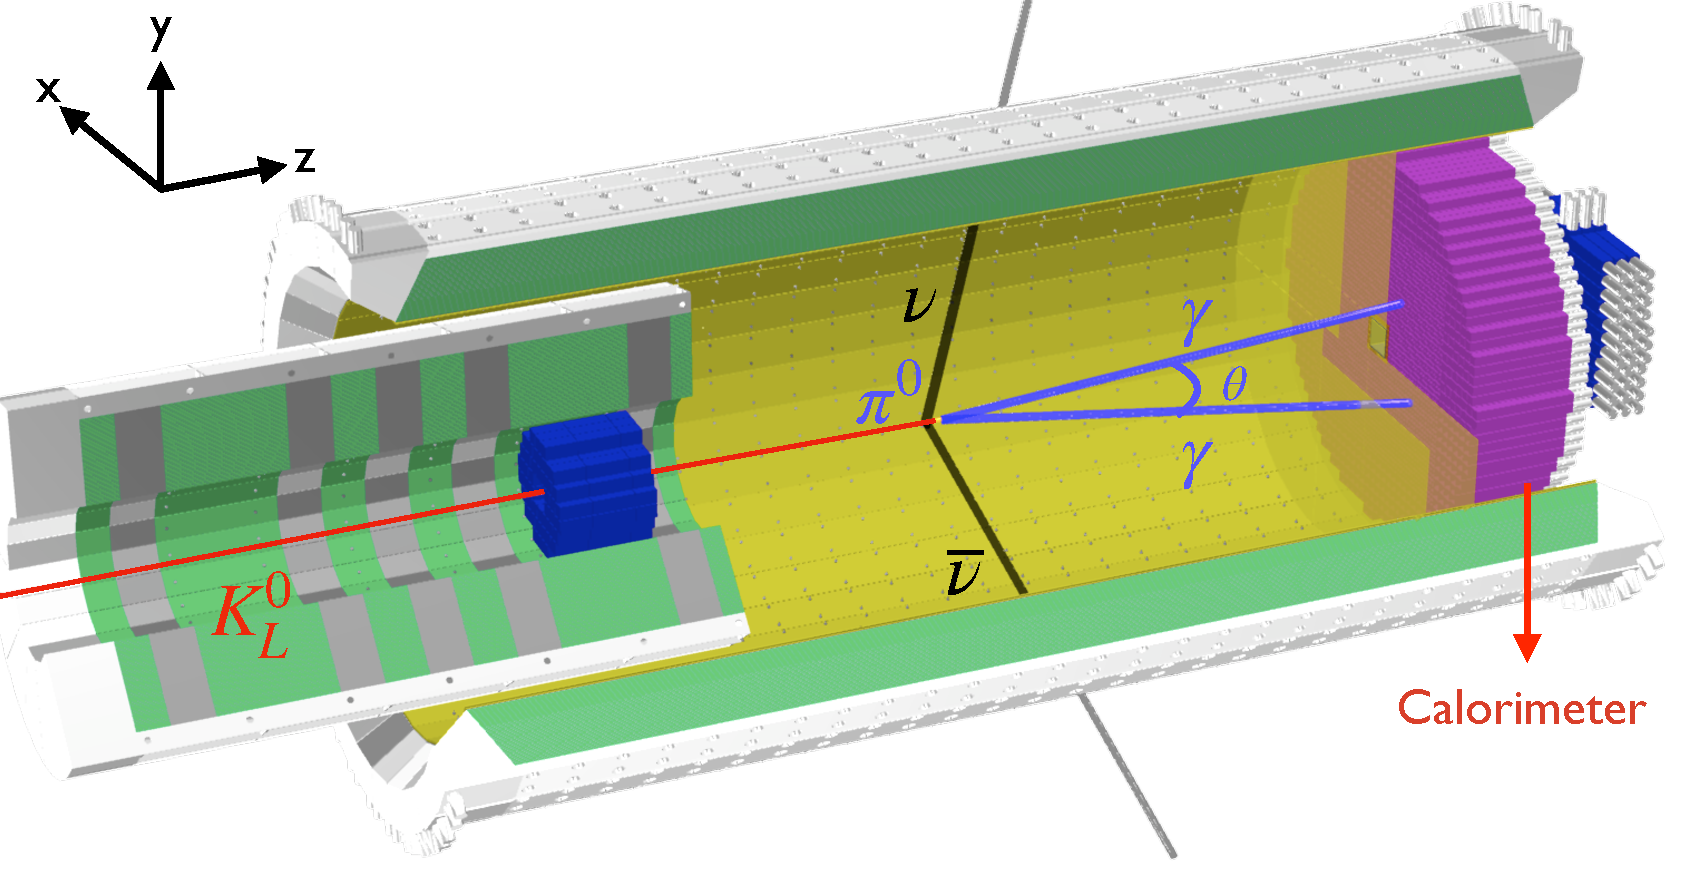
\includegraphics[width=0.8\textwidth]{Figures/Chapter3/Detector_3D.pdf}
\caption{A graphical illustration of a reconstructable ${K_L^0 \to \pi^0 \nu \overline{\nu}}$ decay inside the KOTO detector.}
\label{fig:KOTO_signal_3D}
\end{center}
\end{figure}

%%%
% 3-1-2 major background sources

\subsection{Major background sources}
Any source that can have two hits in the calorimeter potentially mimic signals. By considering the composition of the KOTO beam, the background is primarily induced by $K_L^0$s or neutrons.

\subsubsection{$K_L^0$-induced Background}
Table \ref{tab:KL_decay} lists the main $K_L^0$ decays. Because almost all of the $K_L^0$-decay channels are accompanied by charged particles or more than two photons, the detection of those particles is the most powerful and straightforward approach to suppressing the $K_L^0$ backgrounds. The inefficiency of the detector is essentially translated as the background level. The exception is the $K_L^0\to2\gamma$ decay, which is instead reduced by requiring large $P_T$. 

%In principle, all of them can have two hits in the calorimeter and thus mimic the signals. The suppression of the $K_L^0$-induced backgrounds typically relies on the following approaches: \mynobreakpar

%\begin{itemize}
%\item \textbf{Charge veto}. \\
%The $K_L^0$-decay channels accompanied by charged particles are suppressed by requiring the absence of charged particle hits in the veto system.

%\item \textbf{Photon veto.} \\
%The $K_L^0$-decay channels accompanied by extra photons are suppressed by requiring the absence of photon hits in the veto system.

%\item \textbf{Large $\pi^0$ $P_T$.} \\
%The $K_L^0\to2\gamma$ decay is suppressed by requiring large $P_T$ because there is no any missing particle.

%%%%%%%%%%%%%%%%%%%%%%%%%%%%%
%%% Branching ratio table %%%
%%%
%\end{itemize}

\begin{table} [h]
\centering
\caption{Main $K_L^0$ decays with their branching ratios \parencite{PDG18} . }
\label{tab:KL_decay}
%
\small
\begin{tabular}{l l}
\dtoprule
\rowcolor{LightCyan}
%\mc{1}{Decay mode} & \mc{1}{Branching ratio} \\
Decay mode & Branching ratio \\
\midrule[0.5pt]
$K_L^0 \rightarrow \pi^{\pm} e^{\mp} \nu_e$ ($K_{e3}^0$) & $(40.55 \pm 0.11) \%$ \\
$K_L^0 \rightarrow \pi^{\pm} \mu^{\mp} \nu_{\mu}$ ($K_{\mu 3}^0$) & $(27.04 \pm 0.07) \%$  \\
$K_L^0 \rightarrow 3 \pi^0$ & $(19.52 \pm 0.12) \%$ \\
$K_L^0 \rightarrow \pi^+ \pi^- \pi^0$ & $(12.54 \pm 0.05) \%$  \\
$K_L^0 \rightarrow \pi^{\pm} e^{\mp} \nu_e \gamma$ & $(3.79 \pm 0.06) \times 10^{-3}$ \\
$K_L^0 \rightarrow \pi^+ \pi^-$ & $(1.967 \pm 0.01) \times 10^{-3}$ \\
$K_L^0 \rightarrow \pi^0 \pi^0$ & $(8.64 \pm 0.06) \times 10^{-4}$ \\
$K_L^0 \rightarrow \pi^{\pm} \mu^{\mp} \nu_{\mu} \gamma$ & $(5.65 \pm 0.23) \times 10^{-4}$ \\
$K_L^0 \rightarrow 2 \gamma$ & $(5.47 \pm 0.04) \times 10^{-4}$ \\
\dbottomrule
\end{tabular}
%
\end{table}

%%%%%%%%%%%%%%%%%%

\subsubsection{Neutron-induced Background}

The neutrons from the periphery of the beam (halo neutrons) are also threats. If a neutron hits the detector material, a $\pi^0$ or a $\eta$ might be created through the neutron interactions and decays to two photons hitting the calorimeter. A halo neutron can also enter the calorimeter, two hits might be subsequently generated through the hadronic interactions. Their suppression typically relies on the kinematic variables and the shower shapes.

%----------------------------------------------------------------------------------------
%	SECTION 2: accelerator  
%----------------------------------------------------------------------------------------

\section{Accelerator}

The KOTO experiment is located at Hadron Experimental Facility (HEF) of Japan Proton Accelerator Research Complex (J-PARC) \parencite{JPARC_intro}. The proton beam travels along the orange line in Figure \ref{fig:JPARC_site} before striking the target. Protons are generated at the end of linear particle accelerator (LINAC) \parencite{LINAC}, injected to 3-GeV rapid cycling synchrotron \parencite{RCS},  then accelerated to 30~GeV at main ring synchrotron \parencite{MR}, and eventually delivered to HEF.

\begin{figure}[h]
\begin{center}
\captionsetup{width=.99\linewidth}
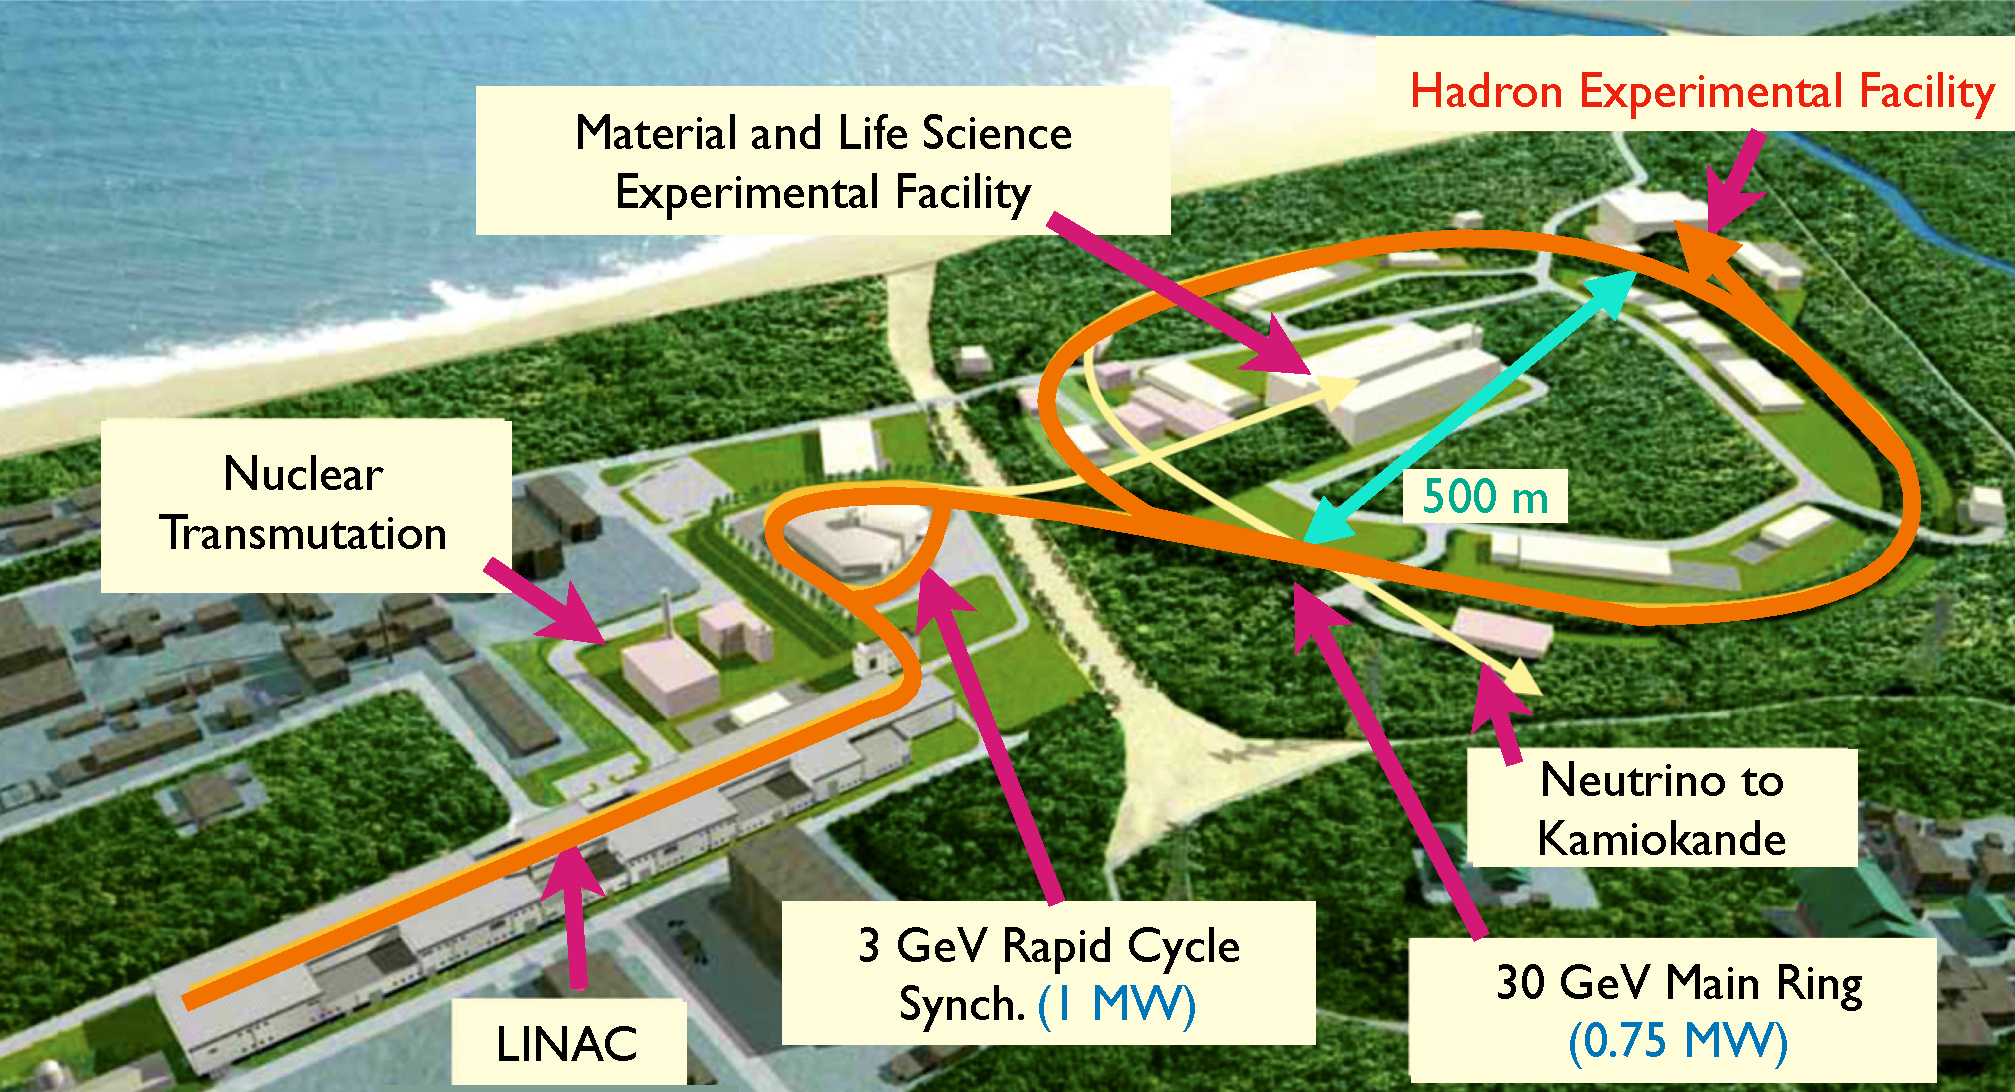
\includegraphics[width=0.75\textwidth]{Figures/Chapter3/JPARC_facility.pdf}
\caption{Entire view of J-PARC (Figure courtesy of \parencite{JPARC_intro} with modifications). The orange line indicates the path of the proton beam.}
\label{fig:JPARC_site}
\end{center}
\end{figure}
 
The proton beam for KOTO is slowly extracted for 2~s and repeated every "spill" of 5.2~s\footnote{The spill length was xxx sec in xxxx and gradually decreased to xxx sec in xxxx.}. Notably, the beam intensity $I=I(t)$ varies with time and the distribution of $I(t)$ is known as the beam structure. The spiky beam structure is not desirable because the instantaneous rate causes the pileup of events, which introduces the signal loss. In order to characterize the beam structure, the flatness level is qualified by the duty factor \parencite{MR}: \mynobreakpar
%
%\vspace{1em}
\begin{align}
\textit{Duty} = \dfrac{\left( \int_{T_1}^{T_2} I(t) dt  \right)^2}{\int_{T_1}^{T_2} dt \int_{T_1}^{T_2} I(t)^2 dt},
\end{align}

\noindent
where $T_1$ and $T_2$ are the times determining the gate width. The duty factor is 100\% if the beam structure is perfectly flat. During the beam operation from 2016 through 2020, the measured duty factor is about 60\%.

%----------------------------------------------------------------------------------------
%	SECTION 3: Detector
%----------------------------------------------------------------------------------------
\section{Detector}

As discussed in Section \ref{sec:basic}, the suppression of $K_L^0$-induced backgrounds strongly relies on the extensive detection of the charged particles and extra photons. The KOTO detector features in the hermetic veto system and the low inefficiency against those particles. Double decay chambers are adopted to identify whether an event is caused by an upstream $K_L^0$ decay. 

Figure \ref{fig:detector} shows an overview of the KOTO detector with the conventional coordinate system. The features of each subdetector are explained as follows.% and summarized in Table~\ref{tab:detector}.
 
%%%
% KOTO detector figure 
%%%
\begin{sidewaysfigure}
\centering
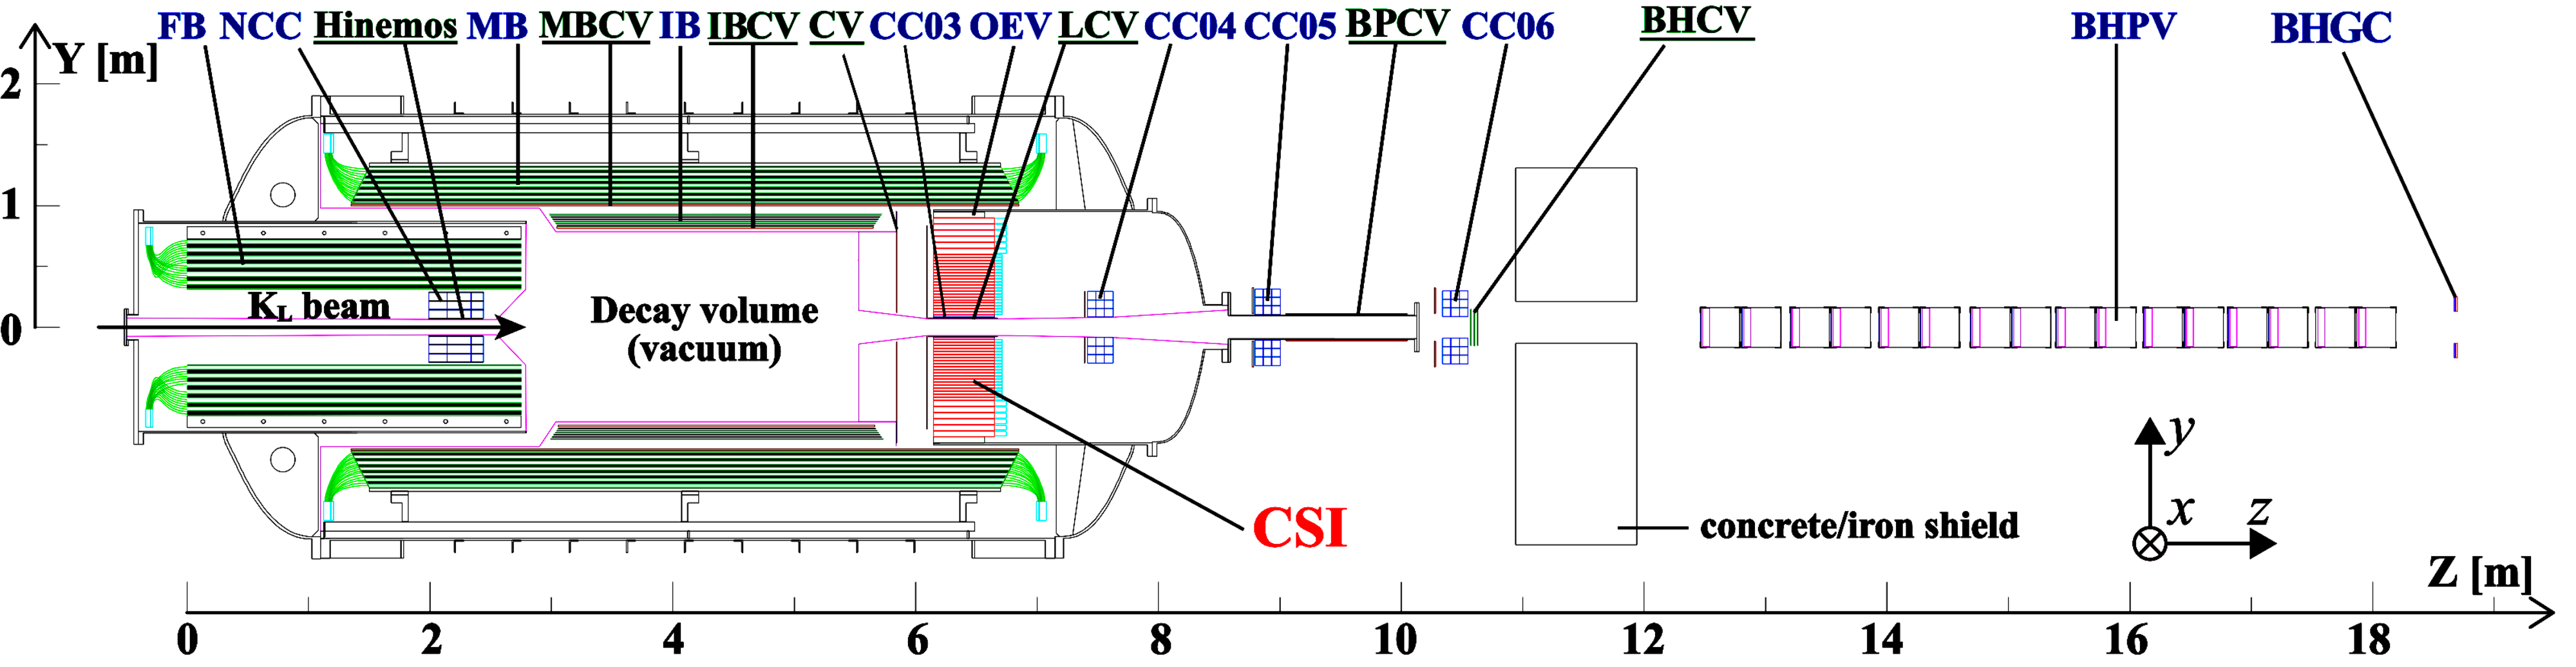
\includegraphics[width=0.99\textwidth]{Figures/Chapter3/KOTODetector2018.pdf}
\caption{Overview of the KOTO Detector. Each subdetector labeled with its abbreviated name in blue (green) is the photon (charged particle) veto counter. The conventional coordinate system of KOTO is displayed.}
\label{fig:detector}
\end{sidewaysfigure}

%%%%%%%%%%%%%%%%%%%%%%%
% KOTO Detector TABLE %
%%%%%%%%%%%%%%%%%%%%%%%
%
%\begin{table}[h]
%\centering
%\begin{small}
%\caption{Summary of the KOTO detector.}
%\label{tab:detector}

%\begin{tabular}{b c c c c}
%\dtoprule
%\rowcolor{LightCyan}
%\mc{1}{Detector} & \mc{1}{Type} & \mc{1}{Purpose} & \mc{1}{Configuration} & \mc{1}{Performance}
% \\
%\midrule[0.5pt]
%CSI  & \makecell{CsI crystals} & \makecell{Photon \\ measurement} & \makecell{Endcap: $z = \SI{6168}{mm}$ \\ Depth: $l = \SI{50}{mm}$ \\ Diameter: $d=\SI{1.9}{m}$ } & \makecell{good} \\ \hline 
%CV   & Plastic scintillator & Charged particle veto & \makecell{Endcap: $z = \SI{6168}{mm}$ \\ Depth: $l = \SI{50}{mm}$ \\ Diameter: $d=\SI{1.9}{m}$ } & good \\ \hline
%NCC  & 3 CsI crystals & suppression & \makecell{Endcap: $z = \SI{6168}{mm}$ \\ Depth: $l = \SI{50}{mm}$ \\ Diameter: $d=\SI{1.9}{m}$ } & good \\ \hline
%Hinemos  & 3 CsI crystals & suppression & \makecell{Endcap: $z = \SI{6168}{mm}$ \\ Depth: $l = \SI{50}{mm}$ \\ Diameter: $d=\SI{1.9}{m}$ } & good \\ \hline
%FBAR & \makecell{Lead-scintillator \\ sandwich} & Photon veto & \makecell{Endcap: $z = \SI{6168}{mm}$ \\ Depth: $l = \SI{50}{mm}$ \\ Diameter: $d=\SI{1.9}{m}$ } & good \\ \hline
%CBAR &  \makecell{Lead-scintillator \\ sandwich} & Photon veto & \makecell{Endcap: $z = \SI{6168}{mm}$ \\ Depth: $l = \SI{50}{mm}$ \\ Diameter: $d=\SI{1.9}{m}$ } & good \\ \hline
%IB   &  \makecell{Lead-scintillator \\ sandwich} & Photon veto & \makecell{Endcap: $z = \SI{6168}{mm}$ \\ Depth: $l = \SI{50}{mm}$ \\ Diameter: $d=\SI{1.9}{m}$ } & good \\ \hline
%MBCV & Plastic Scintillator & Charged particle veto & \makecell{Endcap: $z = \SI{6168}{mm}$ \\ Depth: $l = \SI{50}{mm}$ \\ Diameter: $d=\SI{1.9}{m}$ } & good \\ \hline
%IBCV & Plastic scintillator & Charged particle veto & \makecell{Endcap: $z = \SI{6168}{mm}$ \\ Depth: $l = \SI{50}{mm}$ \\ Diameter: $d=\SI{1.9}{m}$ } & good \\ \hline
%OEV  & test & Photon measurement & \makecell{Endcap: $z = \SI{6168}{mm}$ \\ Depth: $l = \SI{50}{mm}$ \\ Diameter: $d=\SI{1.9}{m}$ } & good \\ \hline
%CC03 & CsI crystals & Photon measurement & \makecell{Endcap: $z = \SI{6168}{mm}$ \\ Depth: $l = \SI{50}{mm}$ \\ Diameter: $d=\SI{1.9}{m}$ } & good \\ \hline
%LCV  & Plastic scintillator & Charged particle veto & \makecell{Endcap: $z = \SI{6168}{mm}$ \\ Depth: $l = \SI{50}{mm}$ \\ Diameter: $d=\SI{1.9}{m}$ } & good \\ \hline
%CC04 & \makecell{CsI crystals \\ Plastic scintillators} & \makecell{photon veto \\ Charged particle veto} & test & good \\ \hline
%CC05 & \makecell{CsI crystals \\ Plastic scintillators} & \makecell{photon veto \\ Charged particle veto} & test & good \\ \hline
%CC06 & \makecell{CsI crystals \\ Plastic scintillators} & \makecell{photon veto \\ Charged particle veto} & test & good \\ \hline
%BPCV & Plastic Scintillator & measurement & \makecell{Endcap: $z = \SI{6168}{mm}$ \\ Depth: $l = \SI{50}{mm}$ \\ Diameter: $d=\SI{1.9}{m}$ } & good \\ \hline
%BHCV & Wire chamber & Photon measurement & \makecell{Endcap: $z = \SI{6168}{mm}$ \\ Depth: $l = \SI{50}{mm}$ \\ Diameter: $d=\SI{1.9}{m}$ } & good \\ \hline
%BHPV & test & Photon measurement &  \makecell{Endcap: $z = \SI{6168}{mm}$ \\ Depth: $l = \SI{50}{mm}$ \\ Diameter: $d=\SI{1.9}{m}$ } & good \\ \hline
%BHGC & \v{C}erenkov counter & Photon veto & \makecell{Endcap: $z = \SI{6168}{mm}$ \\ Depth: $l = \SI{50}{mm}$ \\ Diameter: $d=\SI{1.9}{m}$ } & good \\
%\dbottomrule
%\end{tabular}
%\end{small}
%\end{table}

%%
%% 3-1 vacuum
%%%%%%%%%%%%%%%
\subsection{Vacuum System}
Vacuum is an essential condition to reduce the $\pi^0$ production through the neutron interactions with gas. The high vacuum environment is required to neglect the gas background but introduce the outgassing from the detector material. Consequently, the "membrane" (pink line in Figure~\ref{fig:detector}), which is a thin (0.2~mm) and loss-mass material to eliminate the interactions with particles, is installed to separate the decay region from the detector space. The decay volume is highly evacuated at 5~$\times$~10$^{-5}$~Pa and the rest is maintained at 1~Pa as a buffer. 

%%
%% 3-2 CSI
%%%%%%%%%%%%%%%%%%

\subsection{Electromagnetic Calorimeter}
The electromagnetic calorimeter, which is comprised of 2716 undoped cesium iodide crystals, is primarily utilized to measure the positions and energies of photons for the $\pi^0$ reconstruction \parencite{CSI}. The nickname "CSI" is given according to the material. As Figure~\ref{fig:CSI_config} shows, the 2240 small crystals have a size of 2.5~$\times$~2.5~$\times$~50~cm$^3$ arranged in the inner region, and the 476 large ones have a size of 5.0~$\times$~5.0~$\times$~50~cm$^3$ arranged in the outer region. The depth is corresponding to 27 radiation lengths ($X_0$), which suggests the negligible inefficiency of photon due to punch-through. A square hole is left in the center to keep the calorimeter in a relatively quieter environment. 

\begin{figure}[h]
\begin{center}
\captionsetup{width=.99\linewidth}
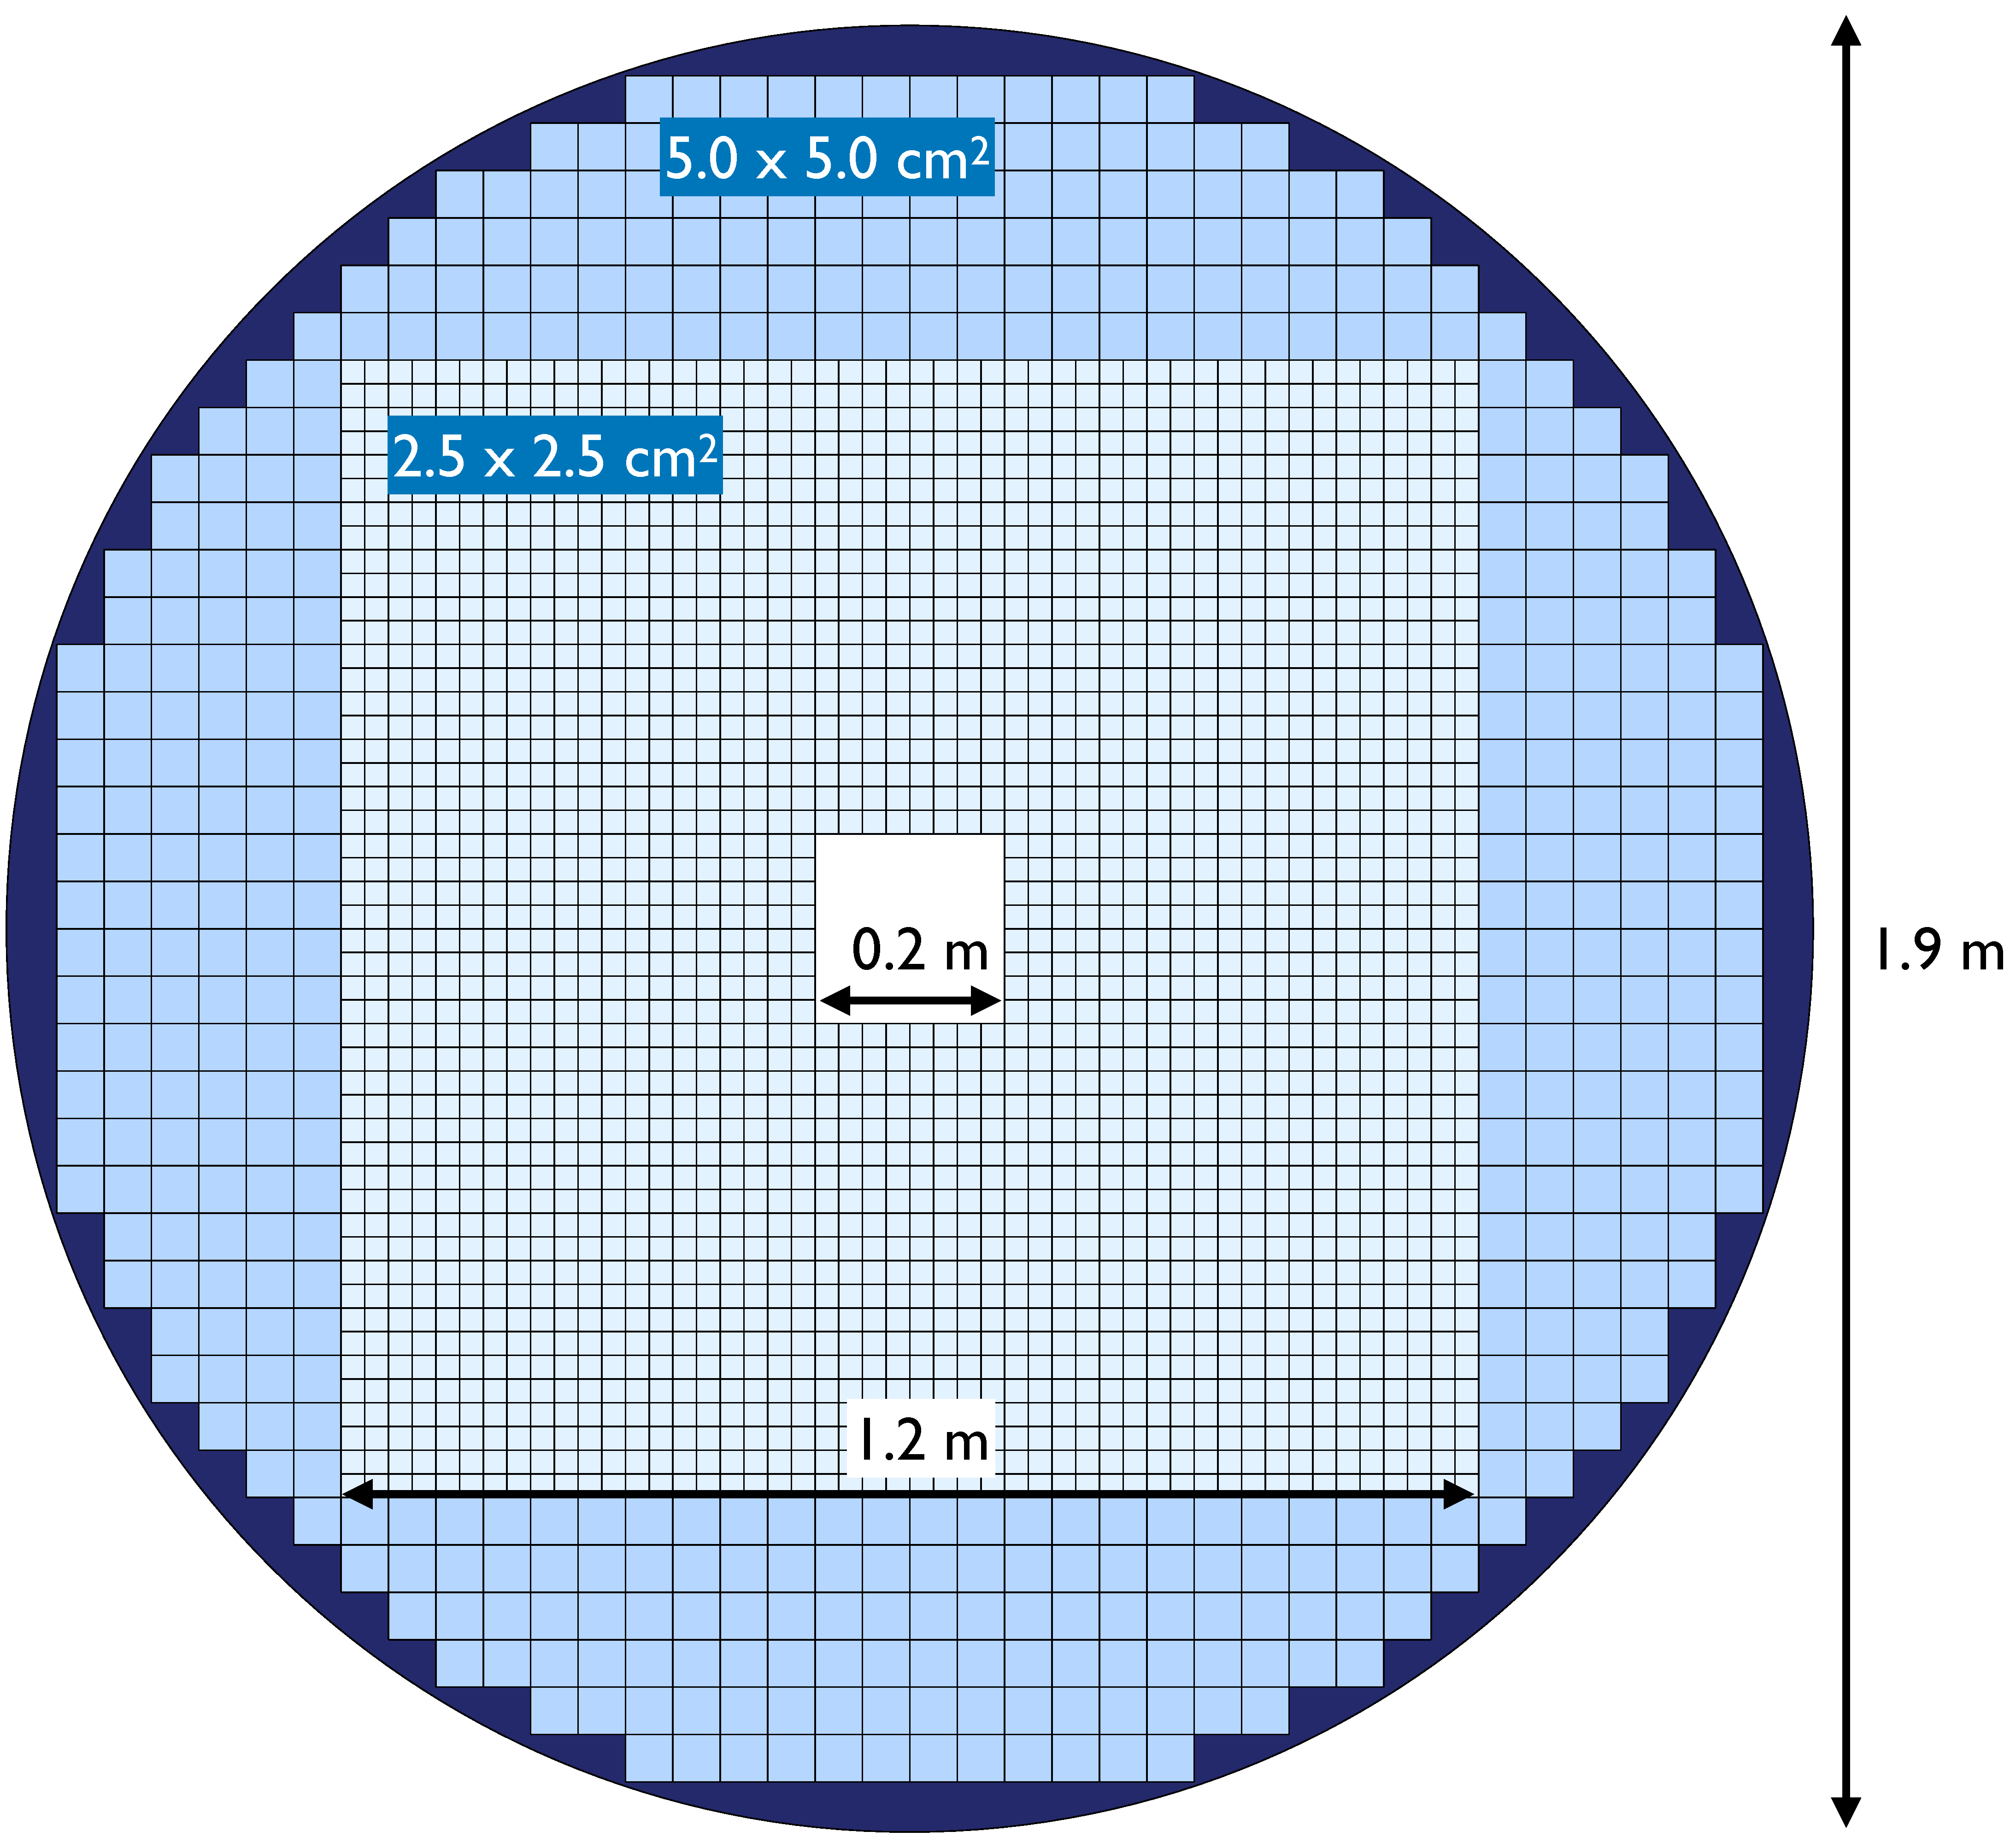
\includegraphics[width=0.6\textwidth]{Figures/Chapter3/CSI_config.pdf}
\caption{An upstream view of the CsI calorimeter \parencite{CSI}.}
\label{fig:CSI_config}
\end{center}
\end{figure}

When a photon hits the calorimeter, the electromagnetic shower is induced and the energy hence spreads out across the adjacent crystals as a cluster. A photomultiplier tube (PMT) is contacted with each crystal for collecting the scintillation lights inside\footnote{A silicone cookie for optical contact \parencite{CSI_cookie} and a UV filter for elimiating the slow components in scintillation lights are inserted between the crystal and the PMT.}. The energy deposit can be obtained by the amount of photo-electrons emitted from the PMT because of the proportionality between two quantities. Moreover, the typical cluster size is characterized by the Mol\`{e}re radius of 3.57~cm \parencite{PDG18}, which is longer than the width of the small crystals. This feature benefits the position resolution and the discrimination power against the shower overlaps.

The performance of the calorimeter is evaluated; for the inner region, the energy resolution is
%
%\vspace{1em}
\begin{align}
\sigma_E / E = \left( 0.66 \oplus 1.81 /\sqrt{E~\text{[GeV]}} \right)~\%, 
\end{align}

\noindent
where $E$ is the total energy and $\oplus$ stands for the quadratic sum, and the position resolution is
%
%\vspace{1em}
\begin{align}
\sigma_{pos} = \left( 1.99 \oplus 3.95 /\sqrt{E~\text{[GeV]}} \right)~\text{mm}.
\end{align}


 
%% 
%% 3-3 CV
%%%%%%%%%%%%%%%%

\subsection{Charge Veto Counter}
If two charged particles in the ${K_L^0 \to \pi^{\pm} e^{\mp} \nu}$ decay hit the calorimeter, two clusters can be generated and misidentified as a $\pi^0$ decay. The Charged Veto counter (CV) \parencite{CV} implemented near the surface of the calorimeter is therefore critical for the detection of the electric charge. Because the ${\mathcal{BR}(K_L^0 \to \pi^{\pm} e^{\mp} \nu)}$ is $\mathcal{O}(1)$, CV is demanded to have a high detection efficiency to charged particles to reduce the ${K_L^0 \to \pi^{\pm} e^{\mp} \nu}$ background by a factor of $\mathcal{O}(10^{11})$. The minimal interaction with hadrons is also essential to avoid introducing extra backgrounds; a halo neutron hits the material and generates $\pi^0$ or $\eta$ that decays to two photons. This suggests the low-mass material for eliminating the $\pi^0$ or $\eta$ productions. 

CV has two layers 251~mm apart. As Figure \ref{fig:CV_config} shows, the upstream (downstream) CV layer has 44 (48) plastic-scintillator strips arranged in four quadrants with a square hole at the center and each strip is attached with wavelength-shifting (WLS) fibers. The orientations of the strips in one layer are arranged perpendicularly to those in the other layer for locating the passage of a charged particle. These materials are sustained by a 0.8-mm-thick carbon fiber reinforced plastic (CFRP) plate.

\begin{figure}[h]
\begin{center}
\captionsetup{width=.99\linewidth}
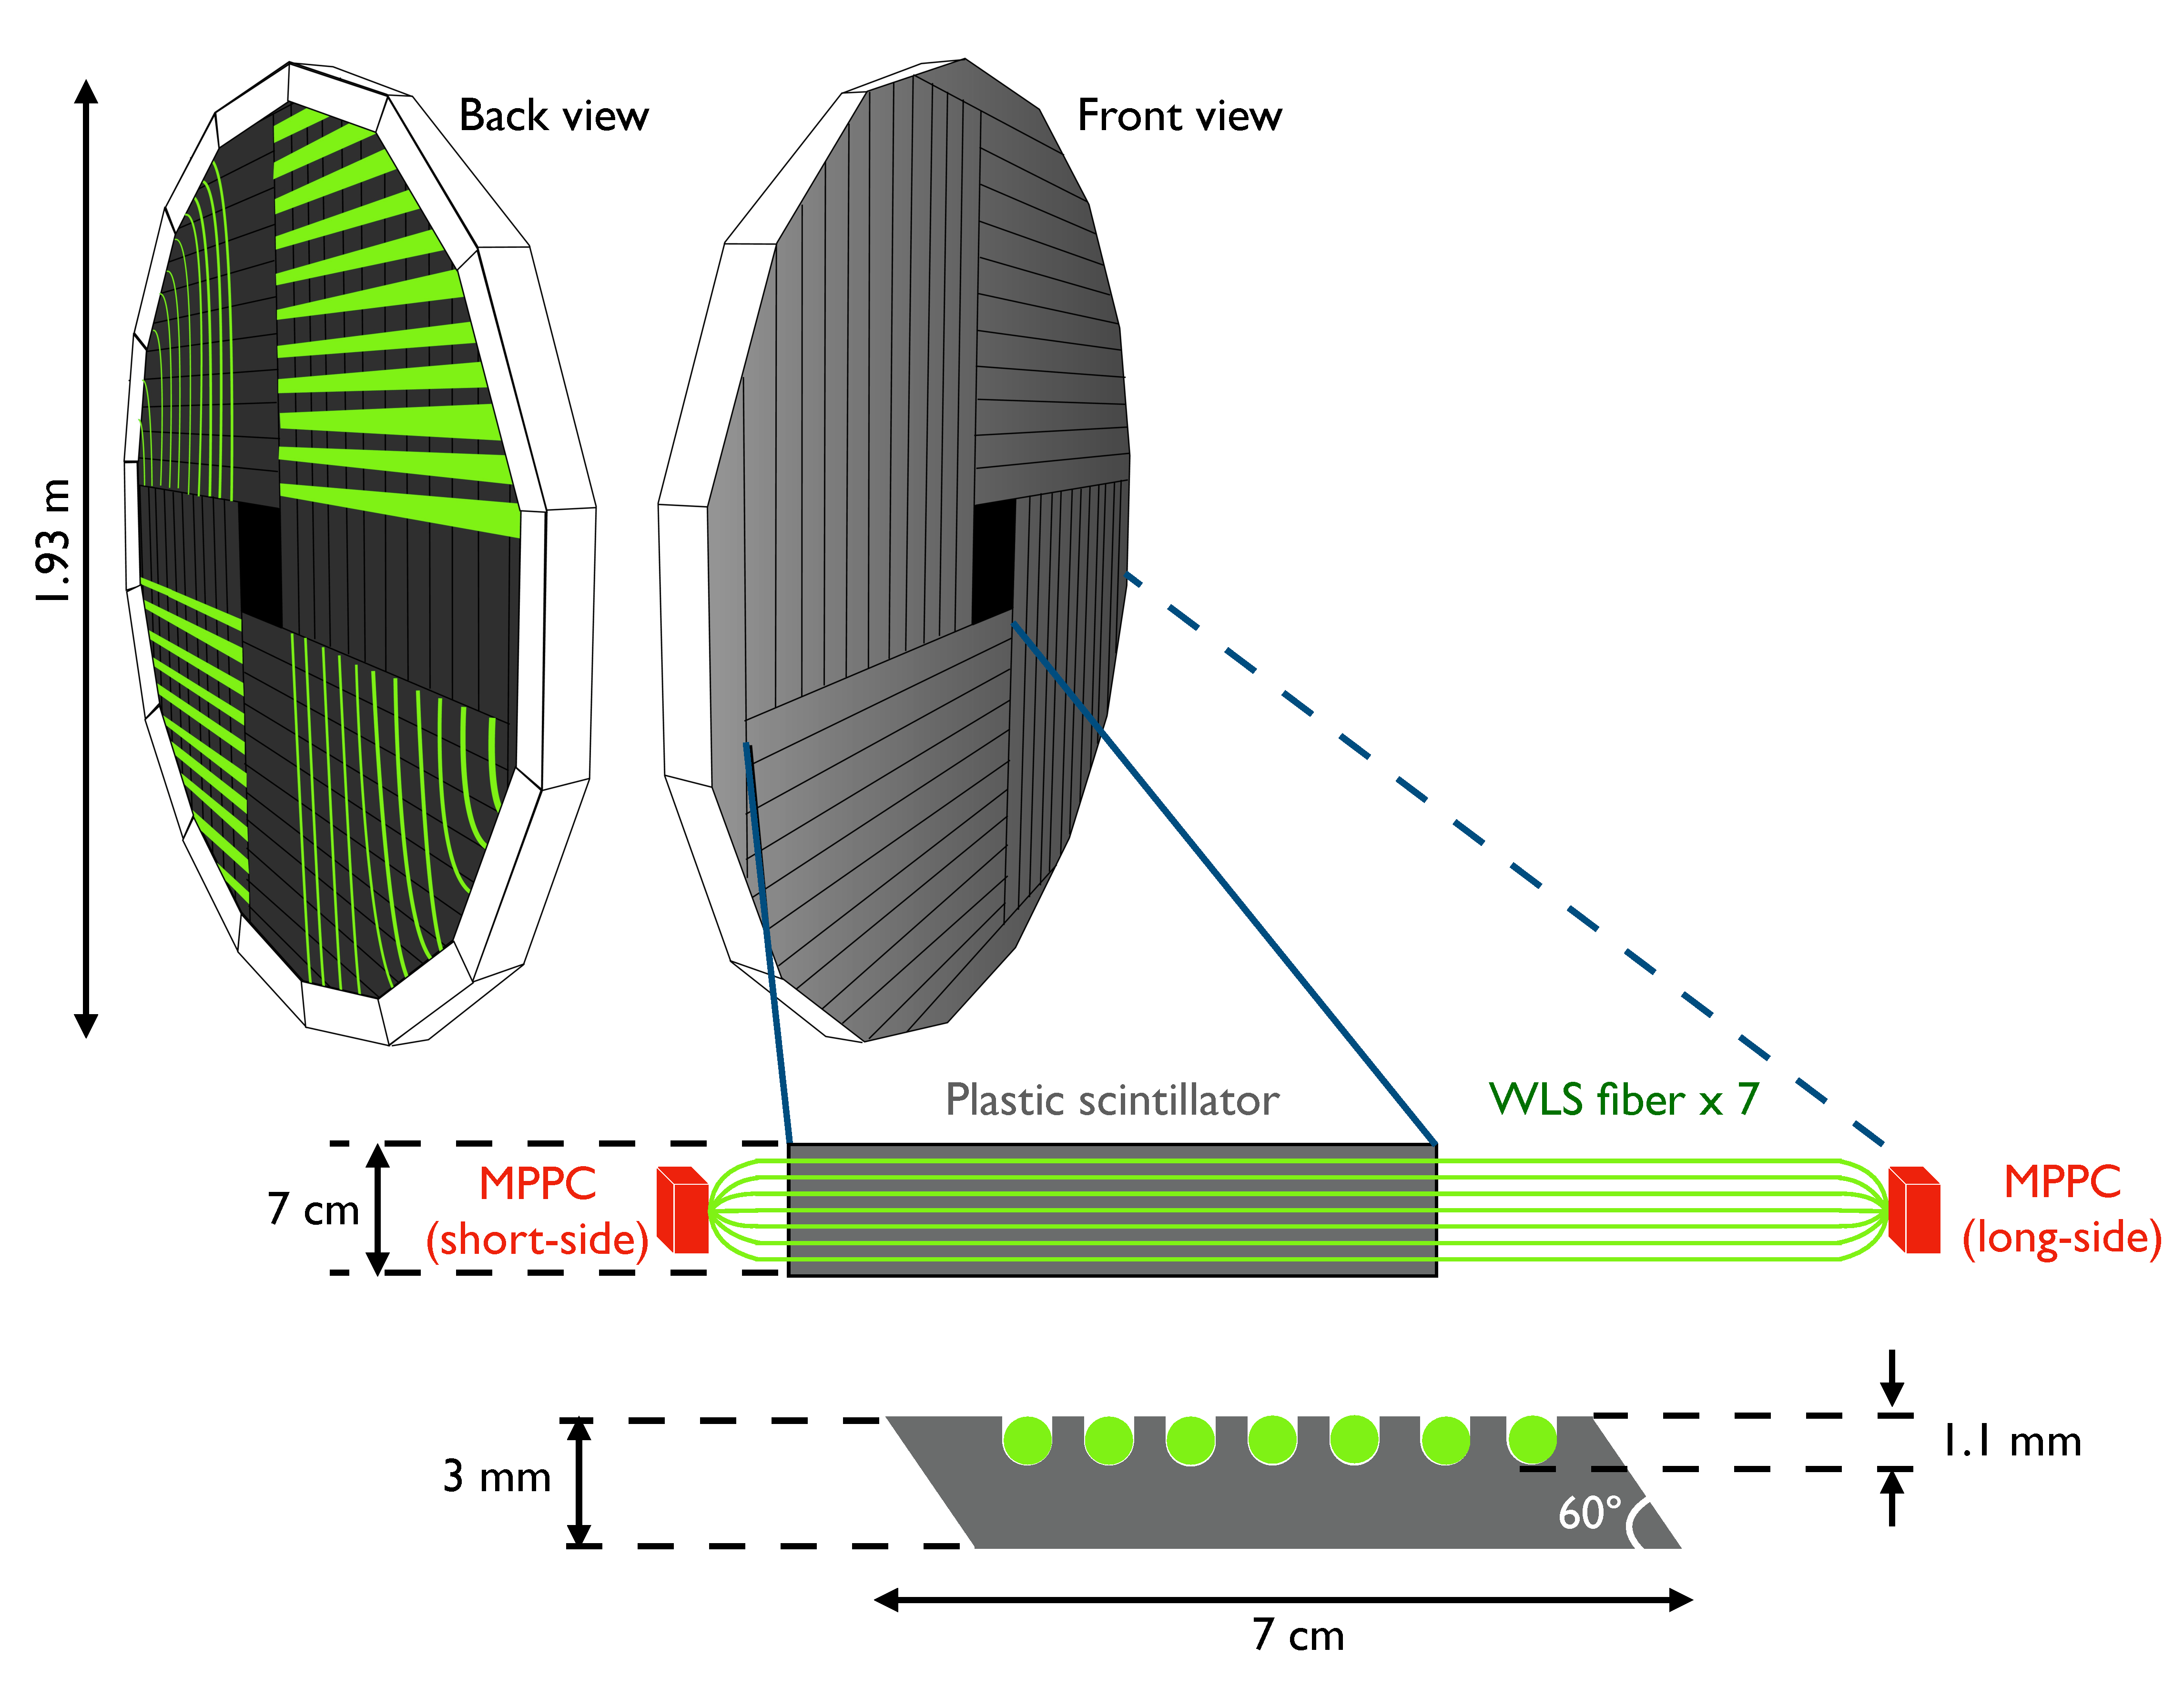
\includegraphics[width=0.99\textwidth]{Figures/Chapter3/CV_config.pdf}
\caption{A schematic diagram of a CV layer \parencite{CV, Maeda}.}
\label{fig:CV_config}
\end{center}
\end{figure}

The energy lost by a charged particle across the medium can yield the scintillation lights through the excitation and deexcitation of an atom. Those lights are guided by fibers and directed to multi-pixel photon counters (MPPC) at both ends. The photo-electrons emitted from MPPC form the pulses, which are used for veto analysis.

By considering the probability of missing two charged particles in both CV layers, the goal of the inefficiency per single layer is $<$ 10$^{-3}$, and the measured value is 1.5~$\times$~10$^{-5}$, which does satisfy the requirement.



%%
%% 3-4 Barrel veto counters
%%%%%%%%%%%%%%%%%%%%%%%%%%%%

\subsection{Barrel Veto Counters}
The ${K_L^0\to\pi^0\pi^0}$ background is considered to be one of the most challenging background sources at KOTO because its reduction principally depends on the detection efficiency to the two additional photons. Because the ${\mathcal{BR}(K_L^0\to\pi^0\pi^0)}$ is $\mathcal{O}(10^{-3})$, the overall photon inefficiency requires to be $<$ 10$^{-4}$ against 100-MeV photons.

The barrel veto counters cylindrically envelop the two decay chambers for detecting additional particles in $K_L^0$ decays: the Front Barrel counter (FB) for the upstream $K_L^0$ decays and the Main Barrel counter (MB) for the fiducial $K_L^0$ decays \parencite{barrel_veto}. Both FB and MB have been initially operated since the first data-taking in 2013. The Inner Barrel counter (IB)  \parencite{IB} was then installed inside MB to improve the detection capability in 2016. Due to the huge coverage, the performance of the barrel system is the leading factor to suppress the ${K_L^0\to\pi^0\pi^0}$ background.

As Figure \ref{fig:barrel_config} shows, FB, MB, and IB are composed of lead-scintillator sandwich and primarily responsible for photon veto. Lead is the dense material selected for the maximal absorption of photons. The lights are emitted by the neighboring scintillators and guided to PMTs by WLS fibers. At the innermost surface of IB and MB, the Inner Barrel Charged Veto counter (IBCV) and the Main Barrel Charged Veto counter (MBCV), which are composed of 10-mm-thick plastic scintillators with WLS fibers, are equipped for the charged particle detection respectively. IBCV covers the inner surface of IB completely while MBCV covers the counterpart of MB in the downstream region of IB. Both avoid the charged particles being absorbed quietly by the material exposed to the decay volume. 

%%% 
\begin{figure}[h]
\begin{center}
\captionsetup{width=.99\linewidth}
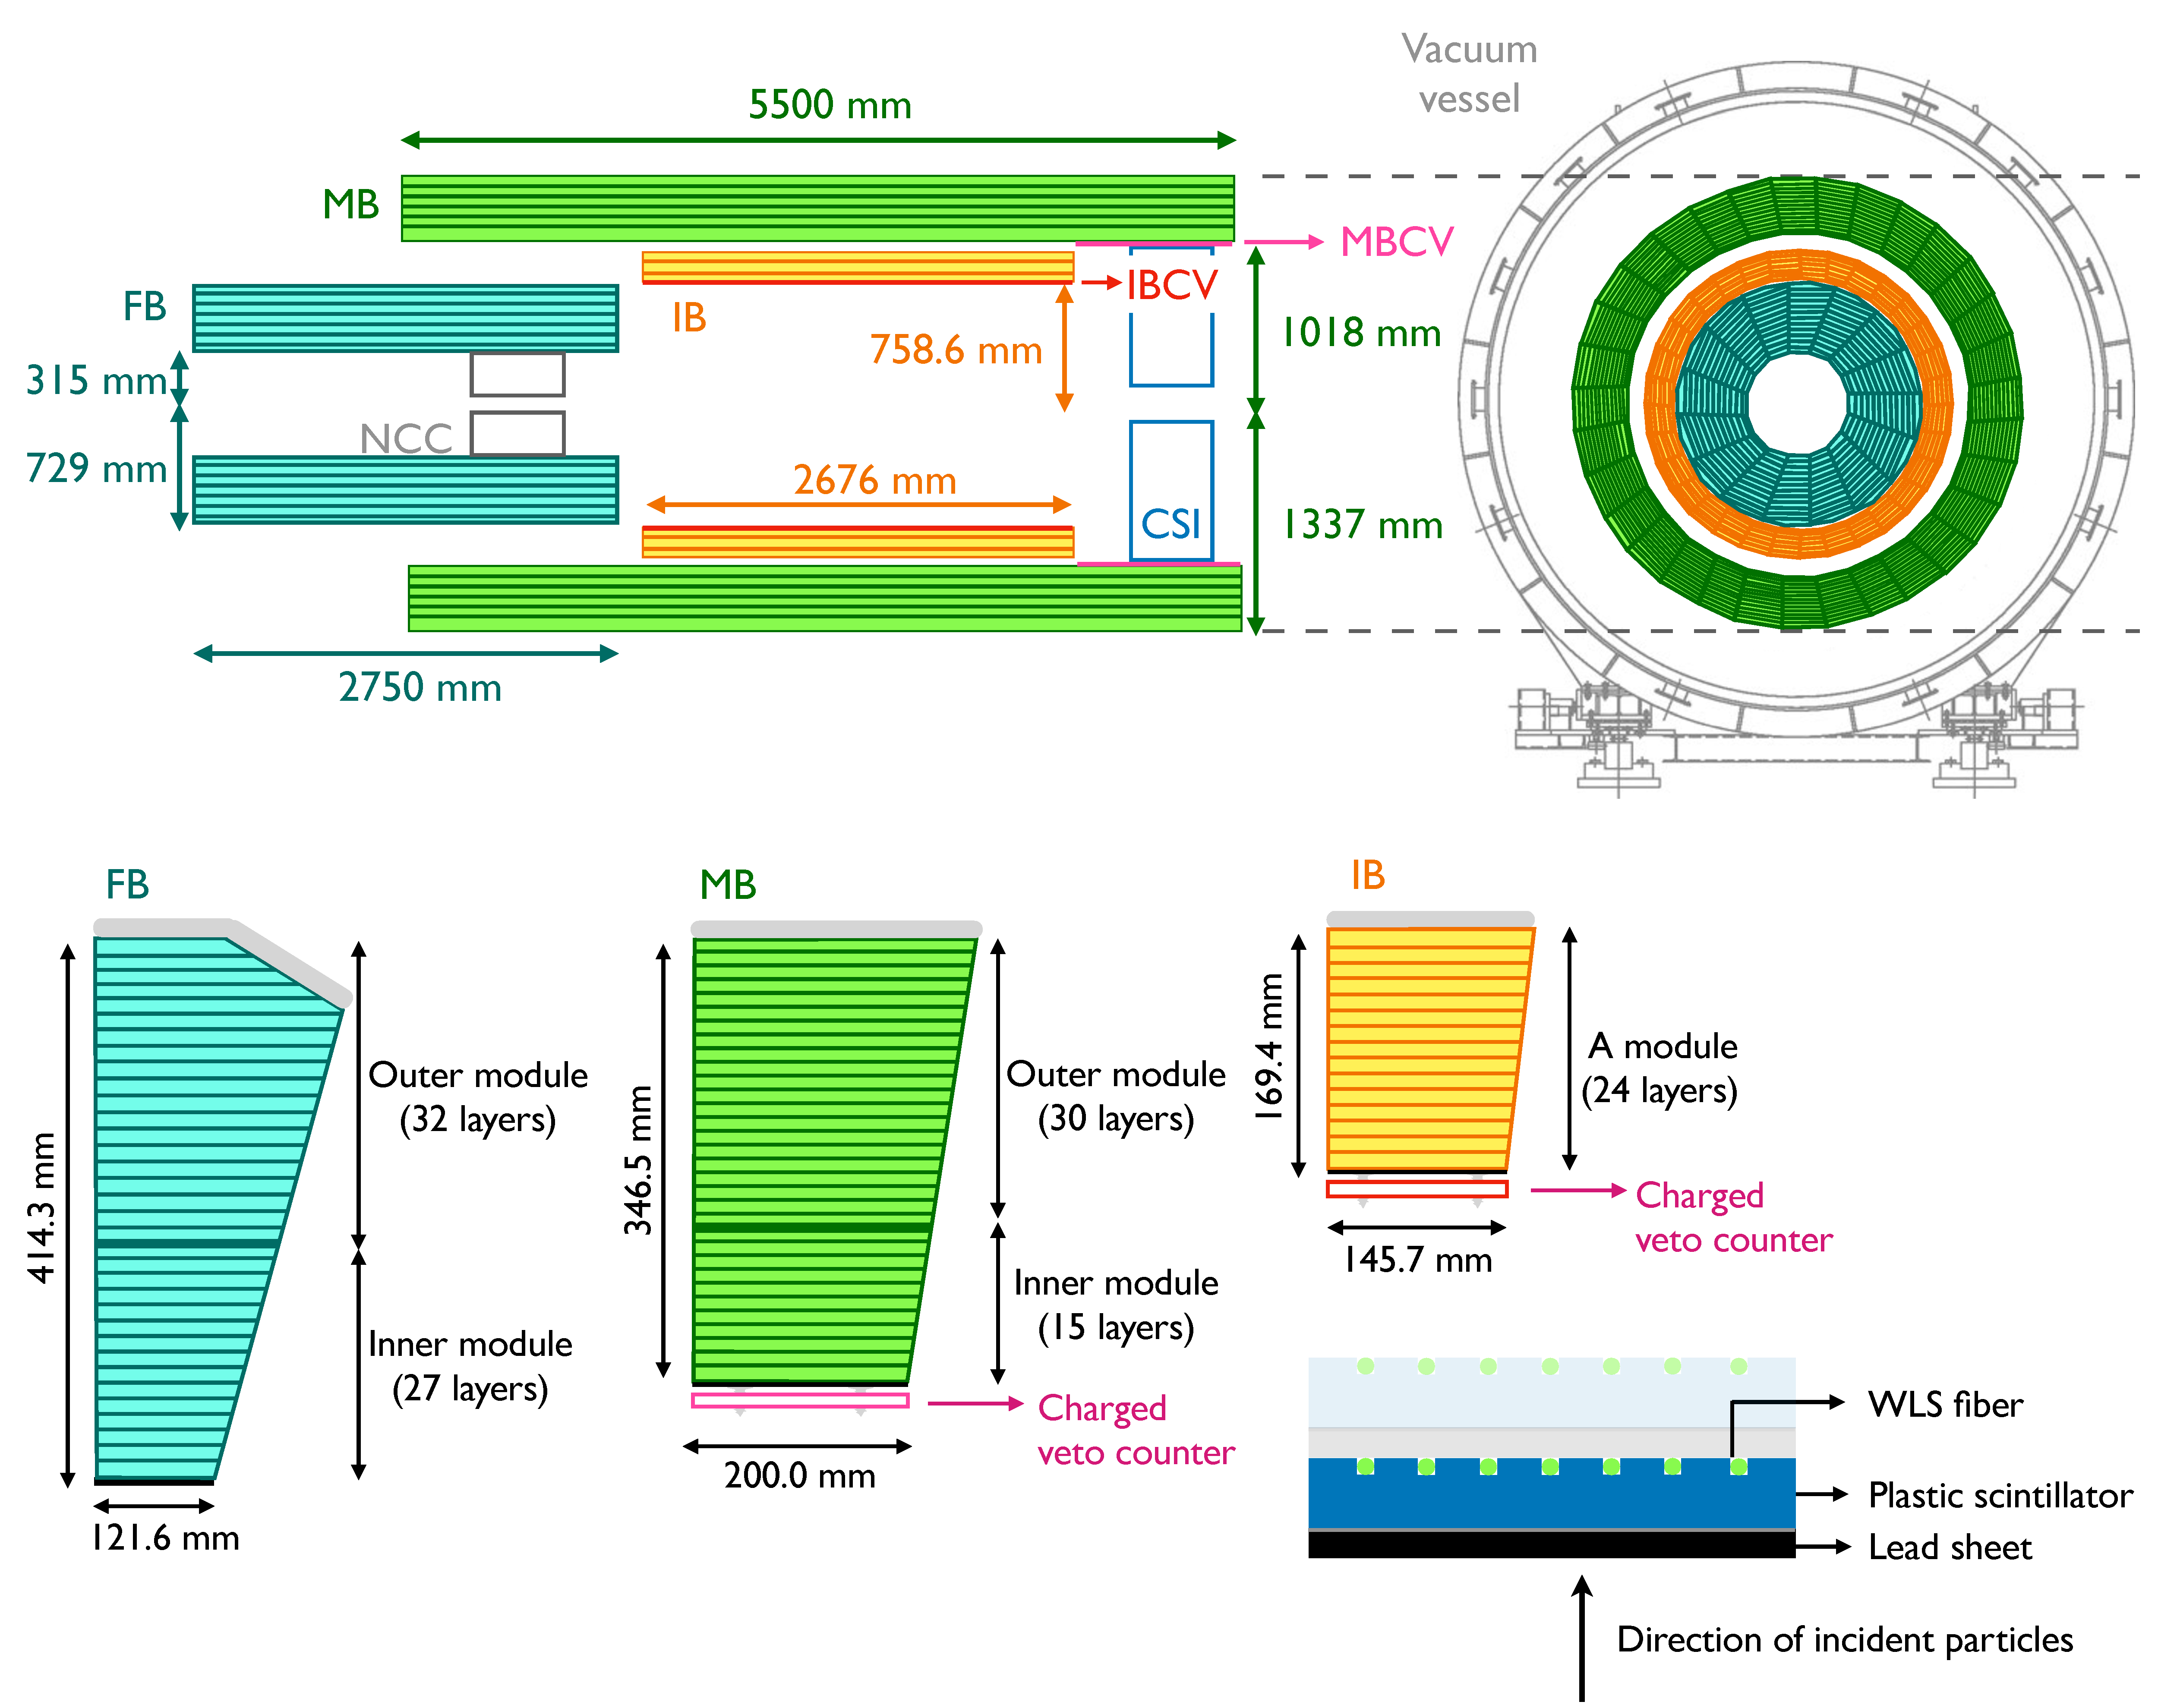
\includegraphics[width=0.99\textwidth]{Figures/Chapter3/Barrel_veto.pdf}
\caption{A schematic diagram of barrel veto counters \parencite{KOTO_intro, barrel_veto, IB}.}
\label{fig:barrel_config}
\end{center}
\end{figure}

The module arrangements and the readout units are summarized in Table~\ref{tab:barrel_property}. Those parameters determine the resolution of a photon hit in barrel veto system: the azimuthal direction by the number of modules, the depth of a photon conversion by the radial segmentation, and the longitudinal direction by the both-end readout. These variables render the background properties analyzable.

%%% barrel parameters %%%
\begin{table}[h]
\centering
\caption{Parameters of the barrel veto counters. }
\label{tab:barrel_property}
%
\small
\begin{tabular}{l c c c}
\dtoprule
\rowcolor{LightCyan}
Subdetector &  Thickness & Module arrangement &  Readout unit\\
\midrule[0.5pt]
FB & 16.5 $X_0$ & \makecell{16 inner modules \\ 16 outer modules} \vspace{0.5em} & \makecell{ Single-end readout \\ 32~$\times$~1~$=$~32~PMTs} \vspace{0.5em} \\
MB & 14.0 $X_0$ & \makecell{32 inner modules \\ 32 outer modules} & \makecell{ Both-end readout \\ 64~$\times$~2~$=$~128 PMTs}  \vspace{0.5em} \\
IB & 5.0 $X_0$ & \makecell{32 modules} & \makecell{ Both-end readout \\ 32~$\times$~2~$=$~64 PMTs } \vspace{0.5em} \\
IBCV & 10~mm & \makecell{32 modules} & \makecell{ Both-end readout \\ 32~$\times$~2~$=$~64~PMTs } \vspace{0.5em} \\
MBCV & 10~mm &  \makecell{16 modules} & \makecell{ Single-end readout \\ 16~$\times$~1~$=$~16~PMTs }\vspace{0.5em} \\
\dbottomrule
\end{tabular}
%
\end{table}

%%
%% 3-5 Neutron collar counter 
%%%%%%%%%%%%%%%%%%%%%%

\subsection{Neutron Collar Counter}
The Neutron Collar Counter (NCC) \parencite{NCC, NCC2} is placed inside the downstream end of FBAR and surrounds the $K_L^0$ beam as an upstream guard of the decay volume. Together with FBAR, the upstream ${K_L^0\to3\pi^0}$ and $K_L^0\to\pi^0\pi^0$ decays can be highly-suppressed. However, as its name hints, halo neutrons can interact with NCC and produce $\pi^0$s decaying to two photons as another background source. If the two photons or other secondary particles in the $\pi^0$ production can be detected in NCC itself, the neutron background is reducible.
 
This is realized by updoped cesium iodide crystals segmented into three parts along the beam direction, as shown in Figure~\ref{fig:NCC_config}. The 4.5~m-long crystals capture the activities inside and transmitted through WLS fibers. Furthermore, The individual readout provides the depth information, which is potentially a variable for the discrimination between photons and neutrons.

\begin{figure}[h]
\begin{center}
\captionsetup{width=.99\linewidth}
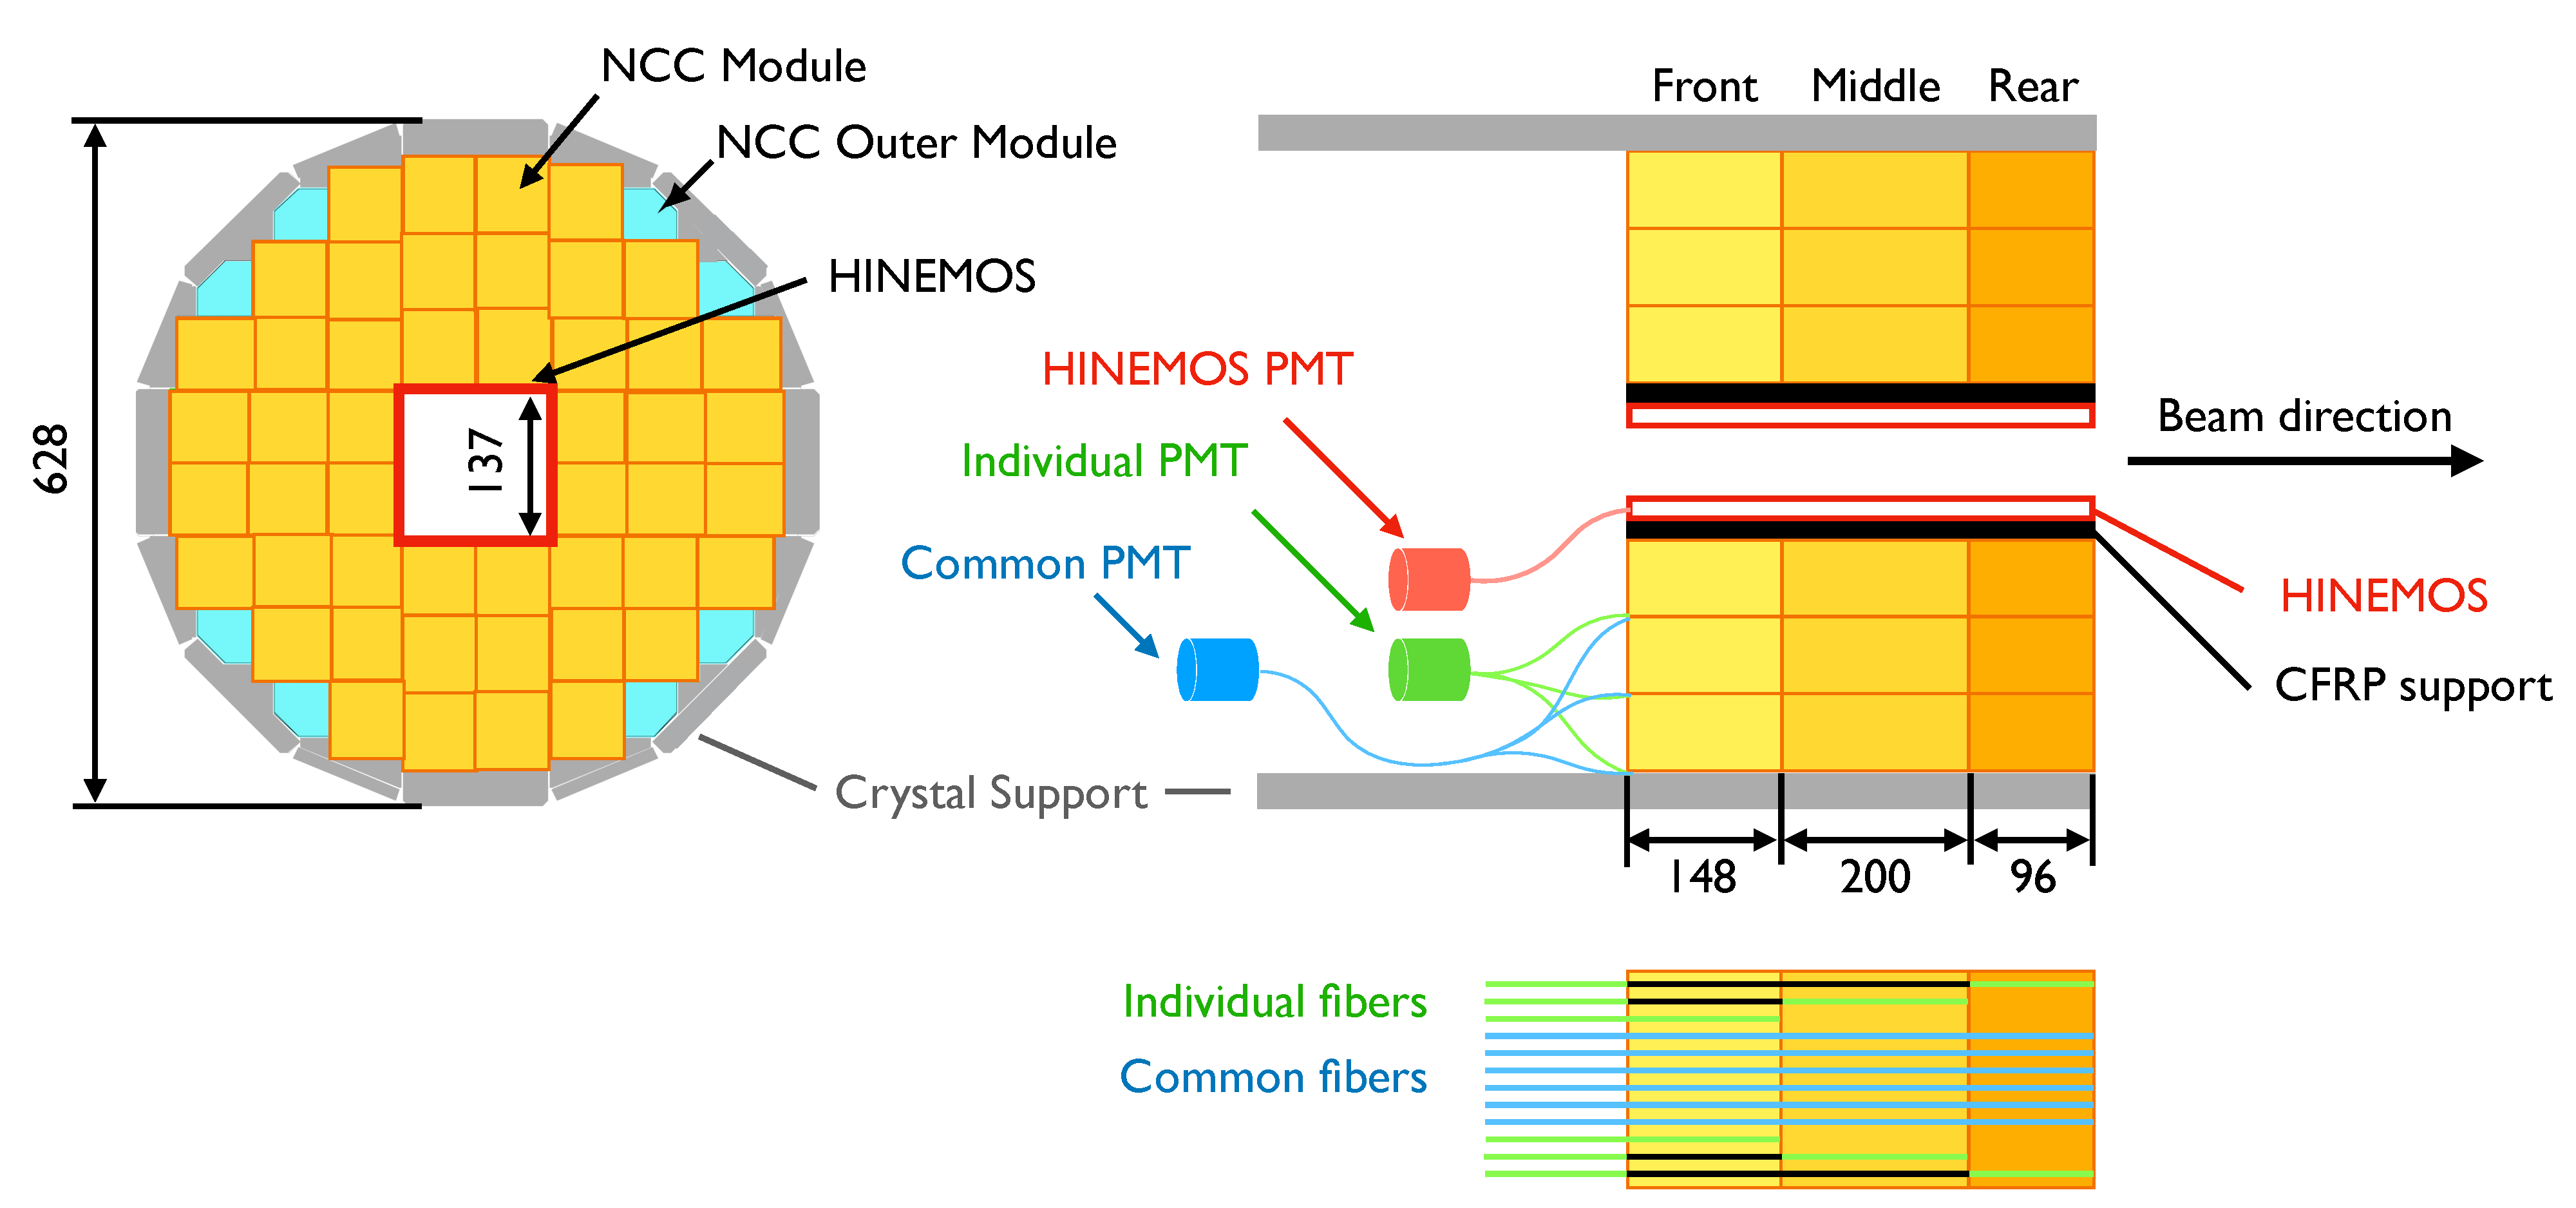
\includegraphics[width=0.99\textwidth]{Figures/Chapter3/NCC_config.pdf}
\caption{A schematic diagram of NCC and HINEMOS \parencite{Maeda, NCC}. The numbers are in the unit of mm.}
\label{fig:NCC_config}
\end{center}
\end{figure}

A $\pi^0$ can also be generated if a $\pi^{\pm}$ penetrates the support installed at the inner surface and undergoes a charge exchange interaction (${\pi^+n \to \pi^0 p}$ or ${\pi^-p \to \pi^0 n}$)\footnote{The source of a single $\pi^{\pm}$ can be produced in the ${K_L^0\to\pi^+\pi^-\pi^0}$ decay at the second collimator. The absence of the coincident hits is expected if other particles do not enter the KOTO detector}. The Horizontal Inner NCC Edge Mounted Scintillator counter (HINEMOS), which consists of four plastic scintillators at the innermost surface, is installed to detect charged particles before the penetration. 

%%
%% 3-6 OEV
%%%%%%%%%%%%%%%%%%%
\subsection{Veto Counters at Outer Edge of the Calorimeter}
The Outer Edge Veto counter (OEV) \parencite{OEV} is composed of 44 lead-scintillator sandwiches with WLS fiber readout. The OEV modules are designed in various shapes appropriately filled in the gap between the cuboid crystals and the cylindrical support of the calorimeter, as shown in Figure~\ref{fig:OEV}. OEV prevents a photon in a $K_L^0$ decay from being absorbed by the support without any detection. 

\begin{figure}[h]
\begin{center}
\captionsetup{width=.99\linewidth}
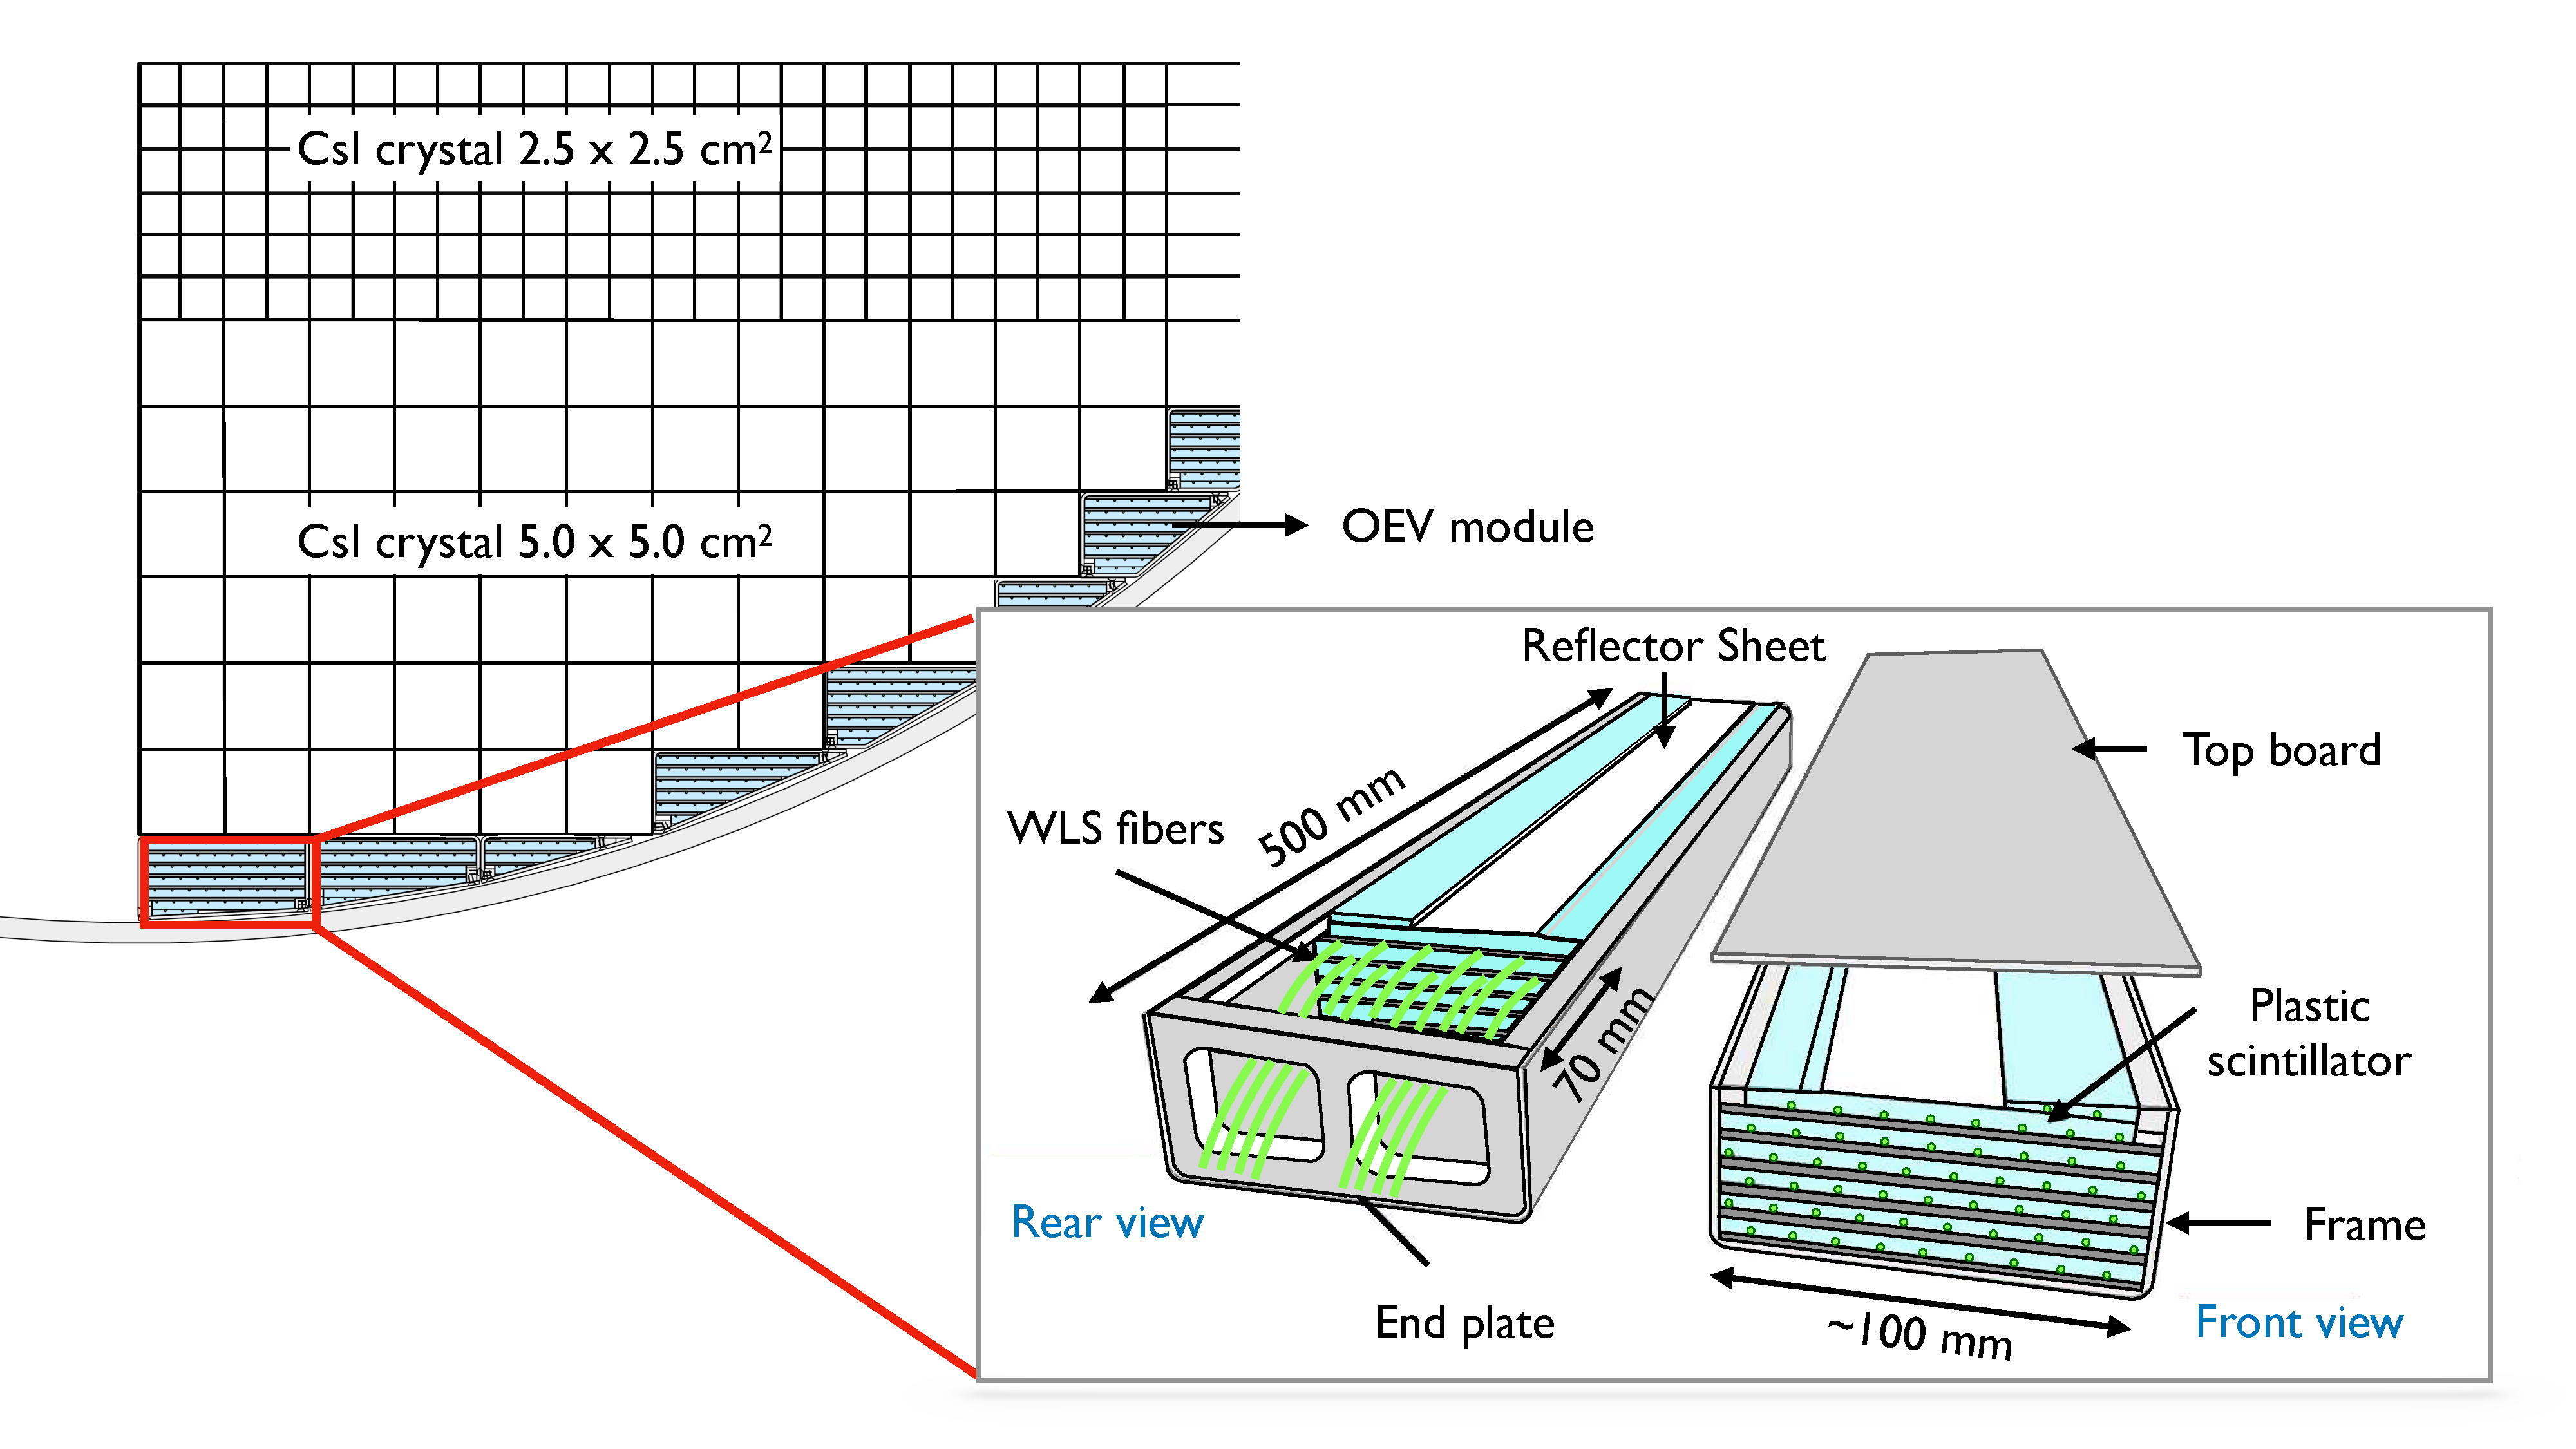
\includegraphics[width=0.99\textwidth]{Figures/Chapter3/OEV_config.pdf}
\caption{A schematic diagram of OEV \parencite{OEV}.}
\label{fig:OEV}
\end{center}
\end{figure}


%%
%% 3-7 CC03, LCV
%%%%%%%%%%%%%%%%%%%%%%

\subsection{Veto Counters inside the Hole of the Calorimeter}
The Collar Counter 3 (CC03) \parencite{CC03} and the Linear Charged Veto counter (LCV) \parencite{LCV} are the square-tube counters inside the hole of the calorimeter for detecting any photons or charged particles hitting around. Figure~\ref{fig:CC03_LCV} shows the configuration of CC03 and LCV. The beam pipe, a 4.5-mm-thick CFRP tube, is installed along the hole for maintaining the whole structure. CC03 consists of sixteen undoped cesium iodide crystals stacked between the calorimeter and the beam pipe. These crystals are not involved in the photon reconstruction in the calorimeter but detects any extra activities near the beam hole. LCV is composed of four 3-mm-thick plastic scintillators embedded with WLS fibers and attached at the inner surface of the beam pipe for detecting a charged particle before entering the beam pipe. Notably, LCV is further extended upstream to CV for the complete coverage.

\begin{figure}[h]
\begin{center}
\captionsetup{width=.99\linewidth}
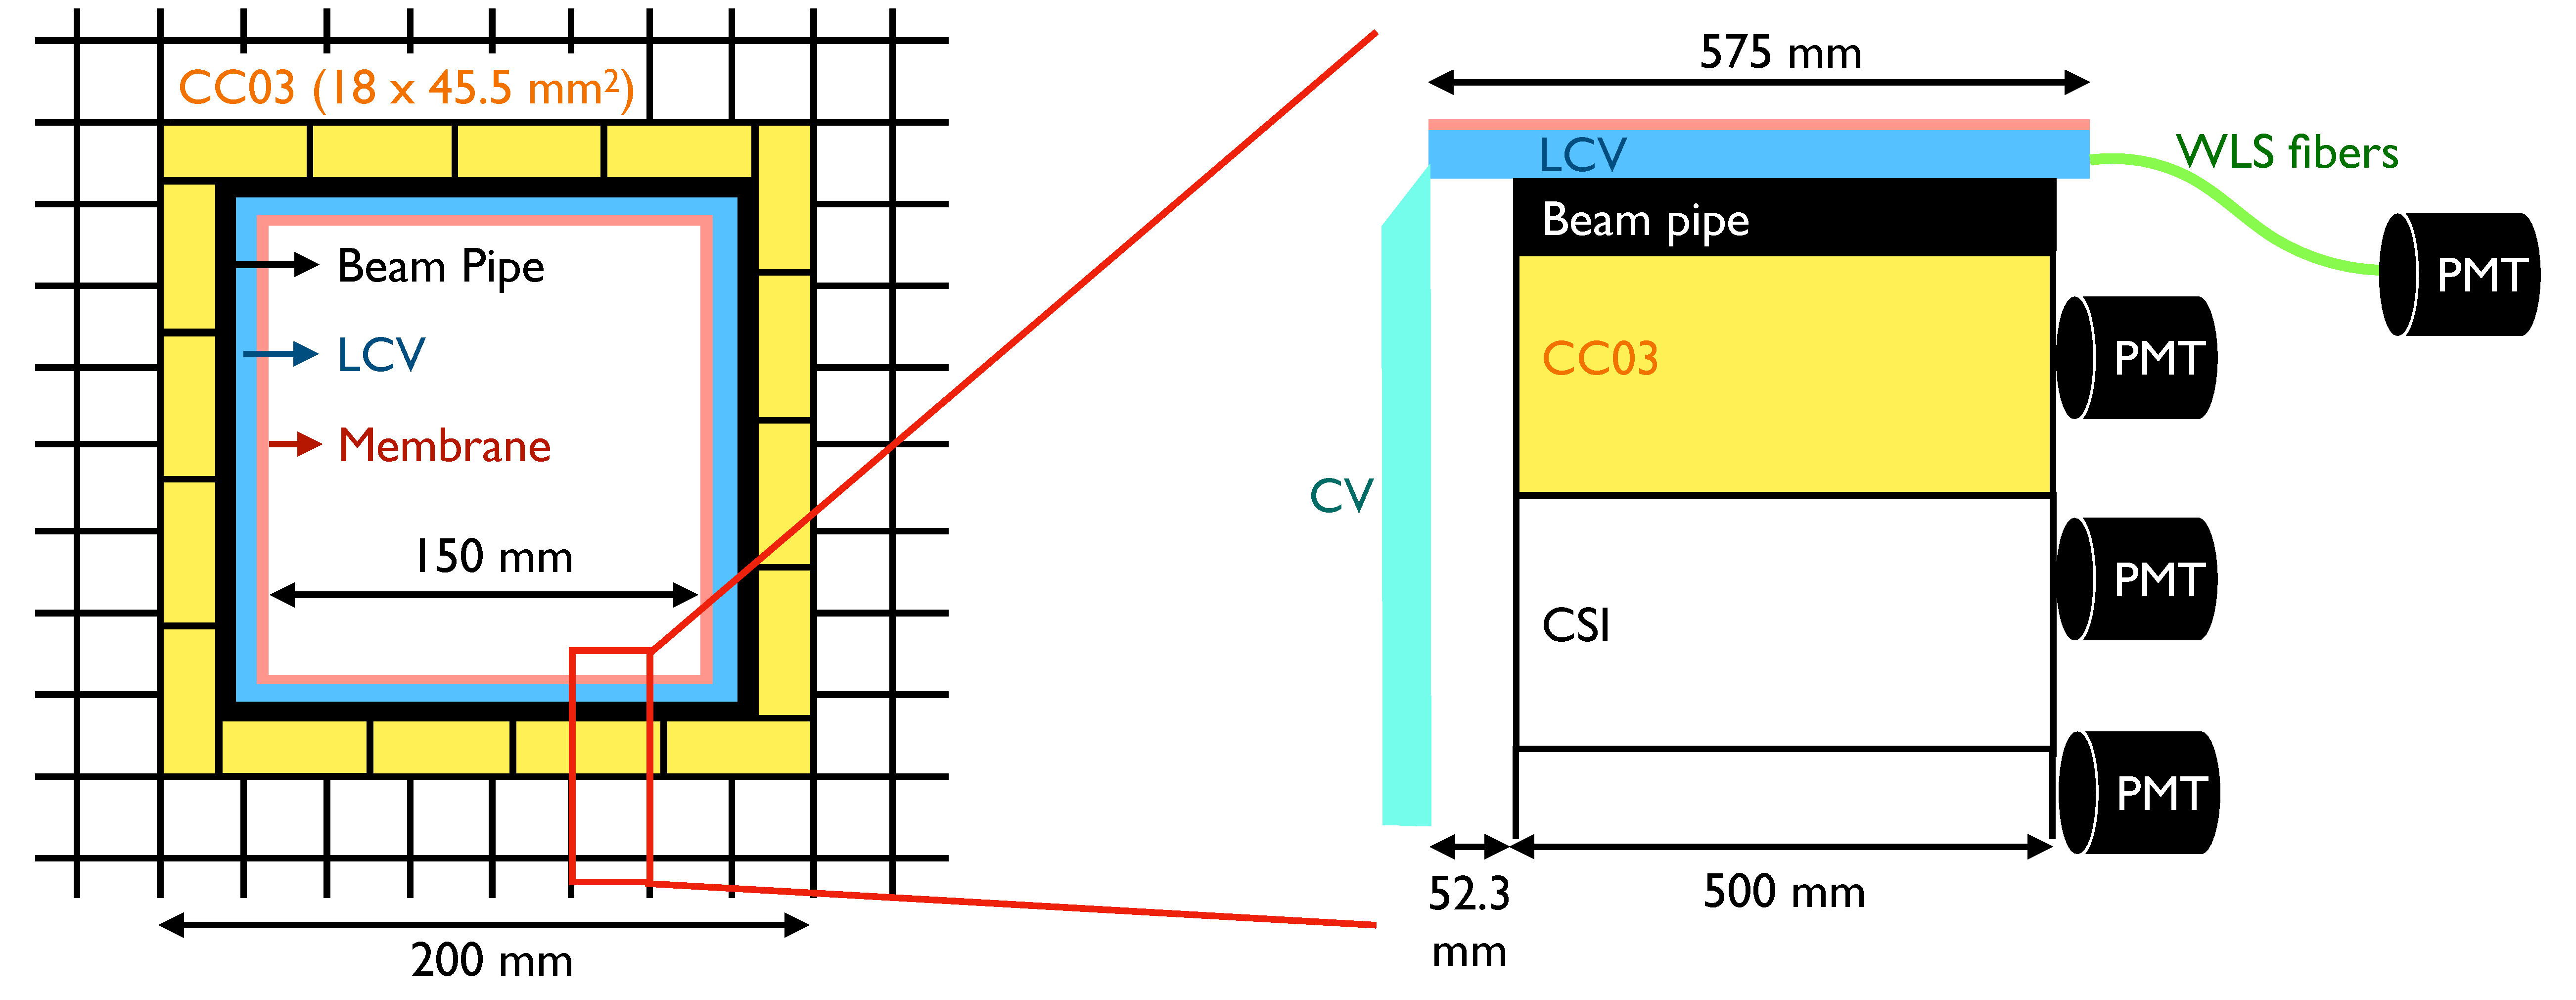
\includegraphics[width=0.85\textwidth]{Figures/Chapter3/CC03_LCV.pdf}
\caption{A schematic diagrams of CC03 and LCV \parencite{Maeda}.}
\label{fig:CC03_LCV}
\end{center}
\end{figure}

%% 
%% 3-8 Downstream collar counter CC04 - CC06
%%%%%%%%%%%%%%%%%%%%%%%%%%%%%%%%%%%%%%%%%%%

\subsection{Downstream Collar Counters}
In the downstream region of the calorimeter, three collar counters, abbreviated as CC04, CC05, and CC06, are installed perpendicularly to the beam direction \parencite{CC04_CC06}.  As Figure~\ref{fig:CC0X} shows, the beam pipe, a 5-mm-thick aluminum square tube, is constructed along the beam hole as an extension of the vacuum environment. CC04 lies inside the vacuum tank, CC05 is installed around the beam pipe, and CC06 is placed in the downstream region of the beam pipe exit. The three collar counters are all composed of undoped Cesium Iodide crystals and the plastic scintillators at upstream surface for detecting photons and charged particles respectively. 

\begin{figure}[H]
\begin{center}
\captionsetup{width=.99\linewidth}
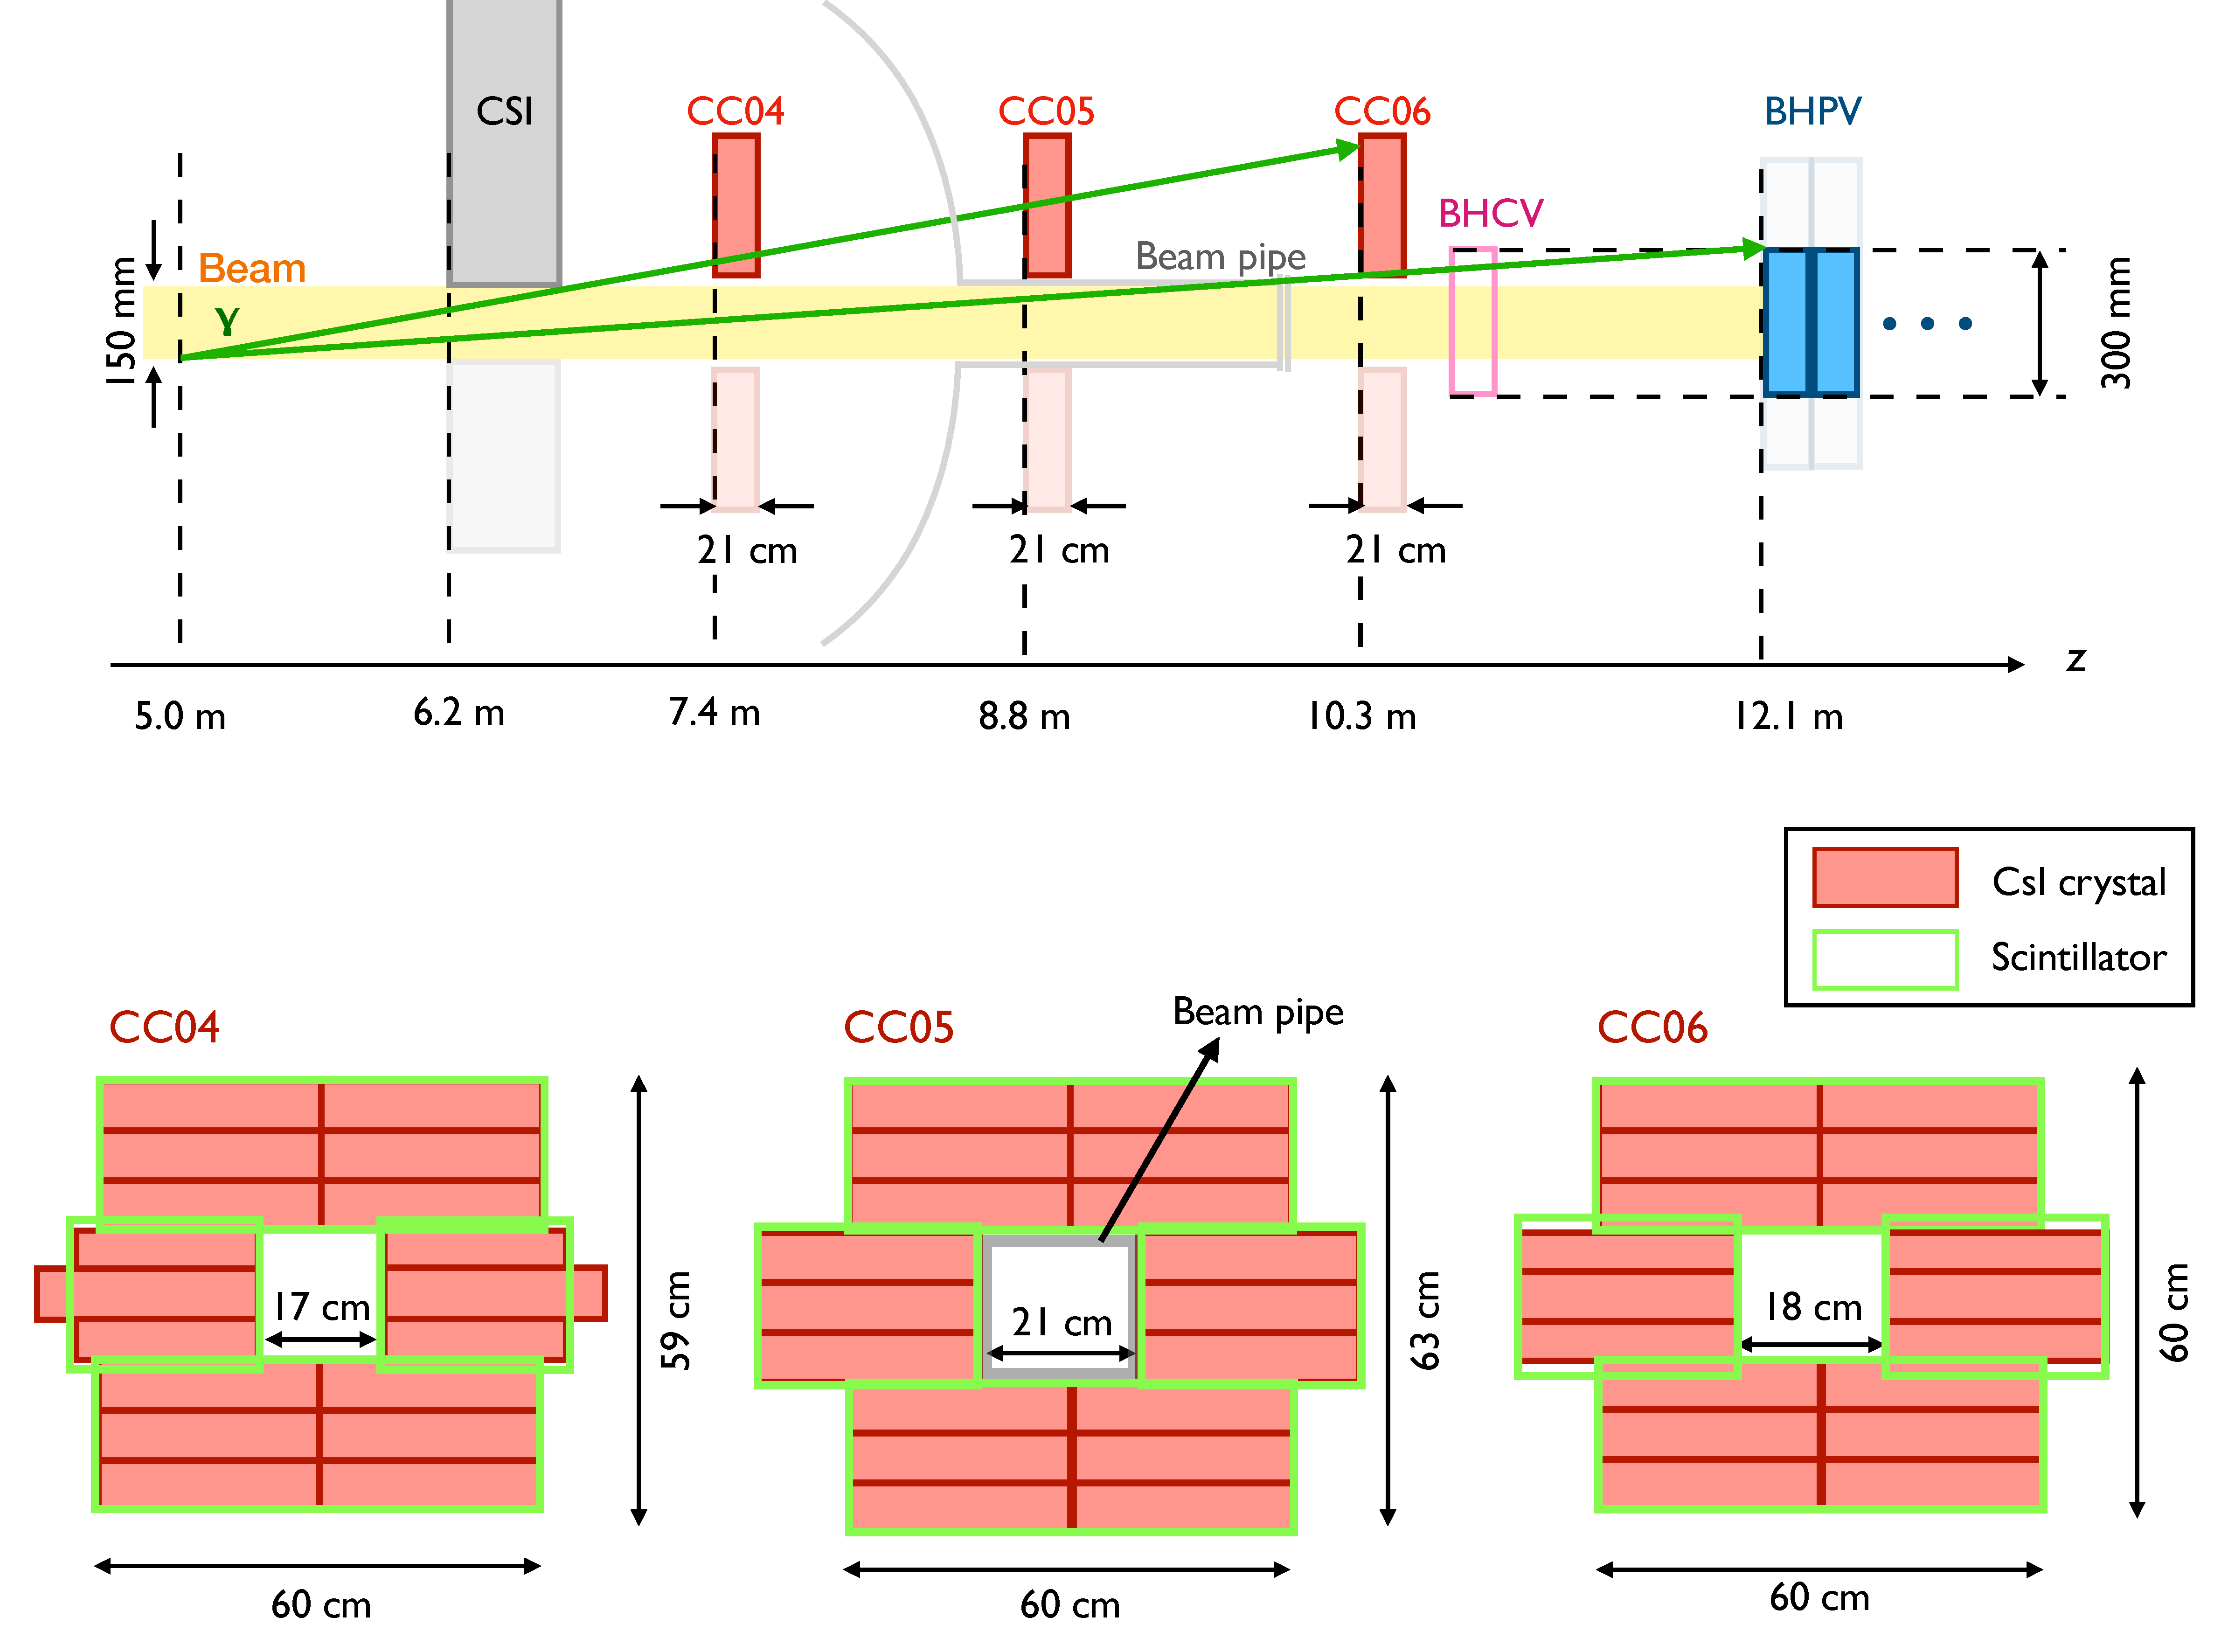
\includegraphics[width=0.99\textwidth]{Figures/Chapter3/CC04_CC06.pdf}
\caption{A schematic diagram of CC04, CC05, and CC06 \parencite{CC04_CC06}. The two green lines indicate the coverage of the downstream counters to a photon from the edge of the beam at z~$=$~5~m. BHPV and BHCV are the in-beam photon and charged particle veto counters respectively (explained in Section~\ref{sec:beam_hole_counter}).} 
\label{fig:CC0X}
\end{center}
\end{figure}

By assuming the downstream boundary of a signal candidate is z~$=$~5~m, the location of CC06 ensures any photon in the ${K_L^0\to\pi^0\pi^0}$ decay escaping into the beam hole can be detected by any of the downstream counters. In line with this, a $\pi^{\pm}$ in the ${K_L^0\to\pi^+\pi^-\pi^0}$ is in general nowhere to escape.

%%
%% 3-9 Beam pipe charge veto (BPCV)
%%%%%%%%%%%%%%%%%%%%%%%%%%%%%%%%%%%%%%%

\subsection{Beam Pipe Charge Veto Counter} 

The ${K_L^0\to\pi^+\pi^-\pi^0}$ decay can be a serious background source if the $\pi^{\pm}$s are absorbed by the beam pipe before entering CC06. The Beam Pipe Charge Veto (BPCV) counter \parencite{BPCV}, which is composed of four 5-mm-thick plastic scintillators surrounding the beam pipe, is therefore implemented to further enhance the detection capability of $\pi^{\pm}$s, as shown in Figure \ref{fig:BPCV}. 

\begin{figure}[H]
\begin{center}
\captionsetup{width=.99\linewidth}
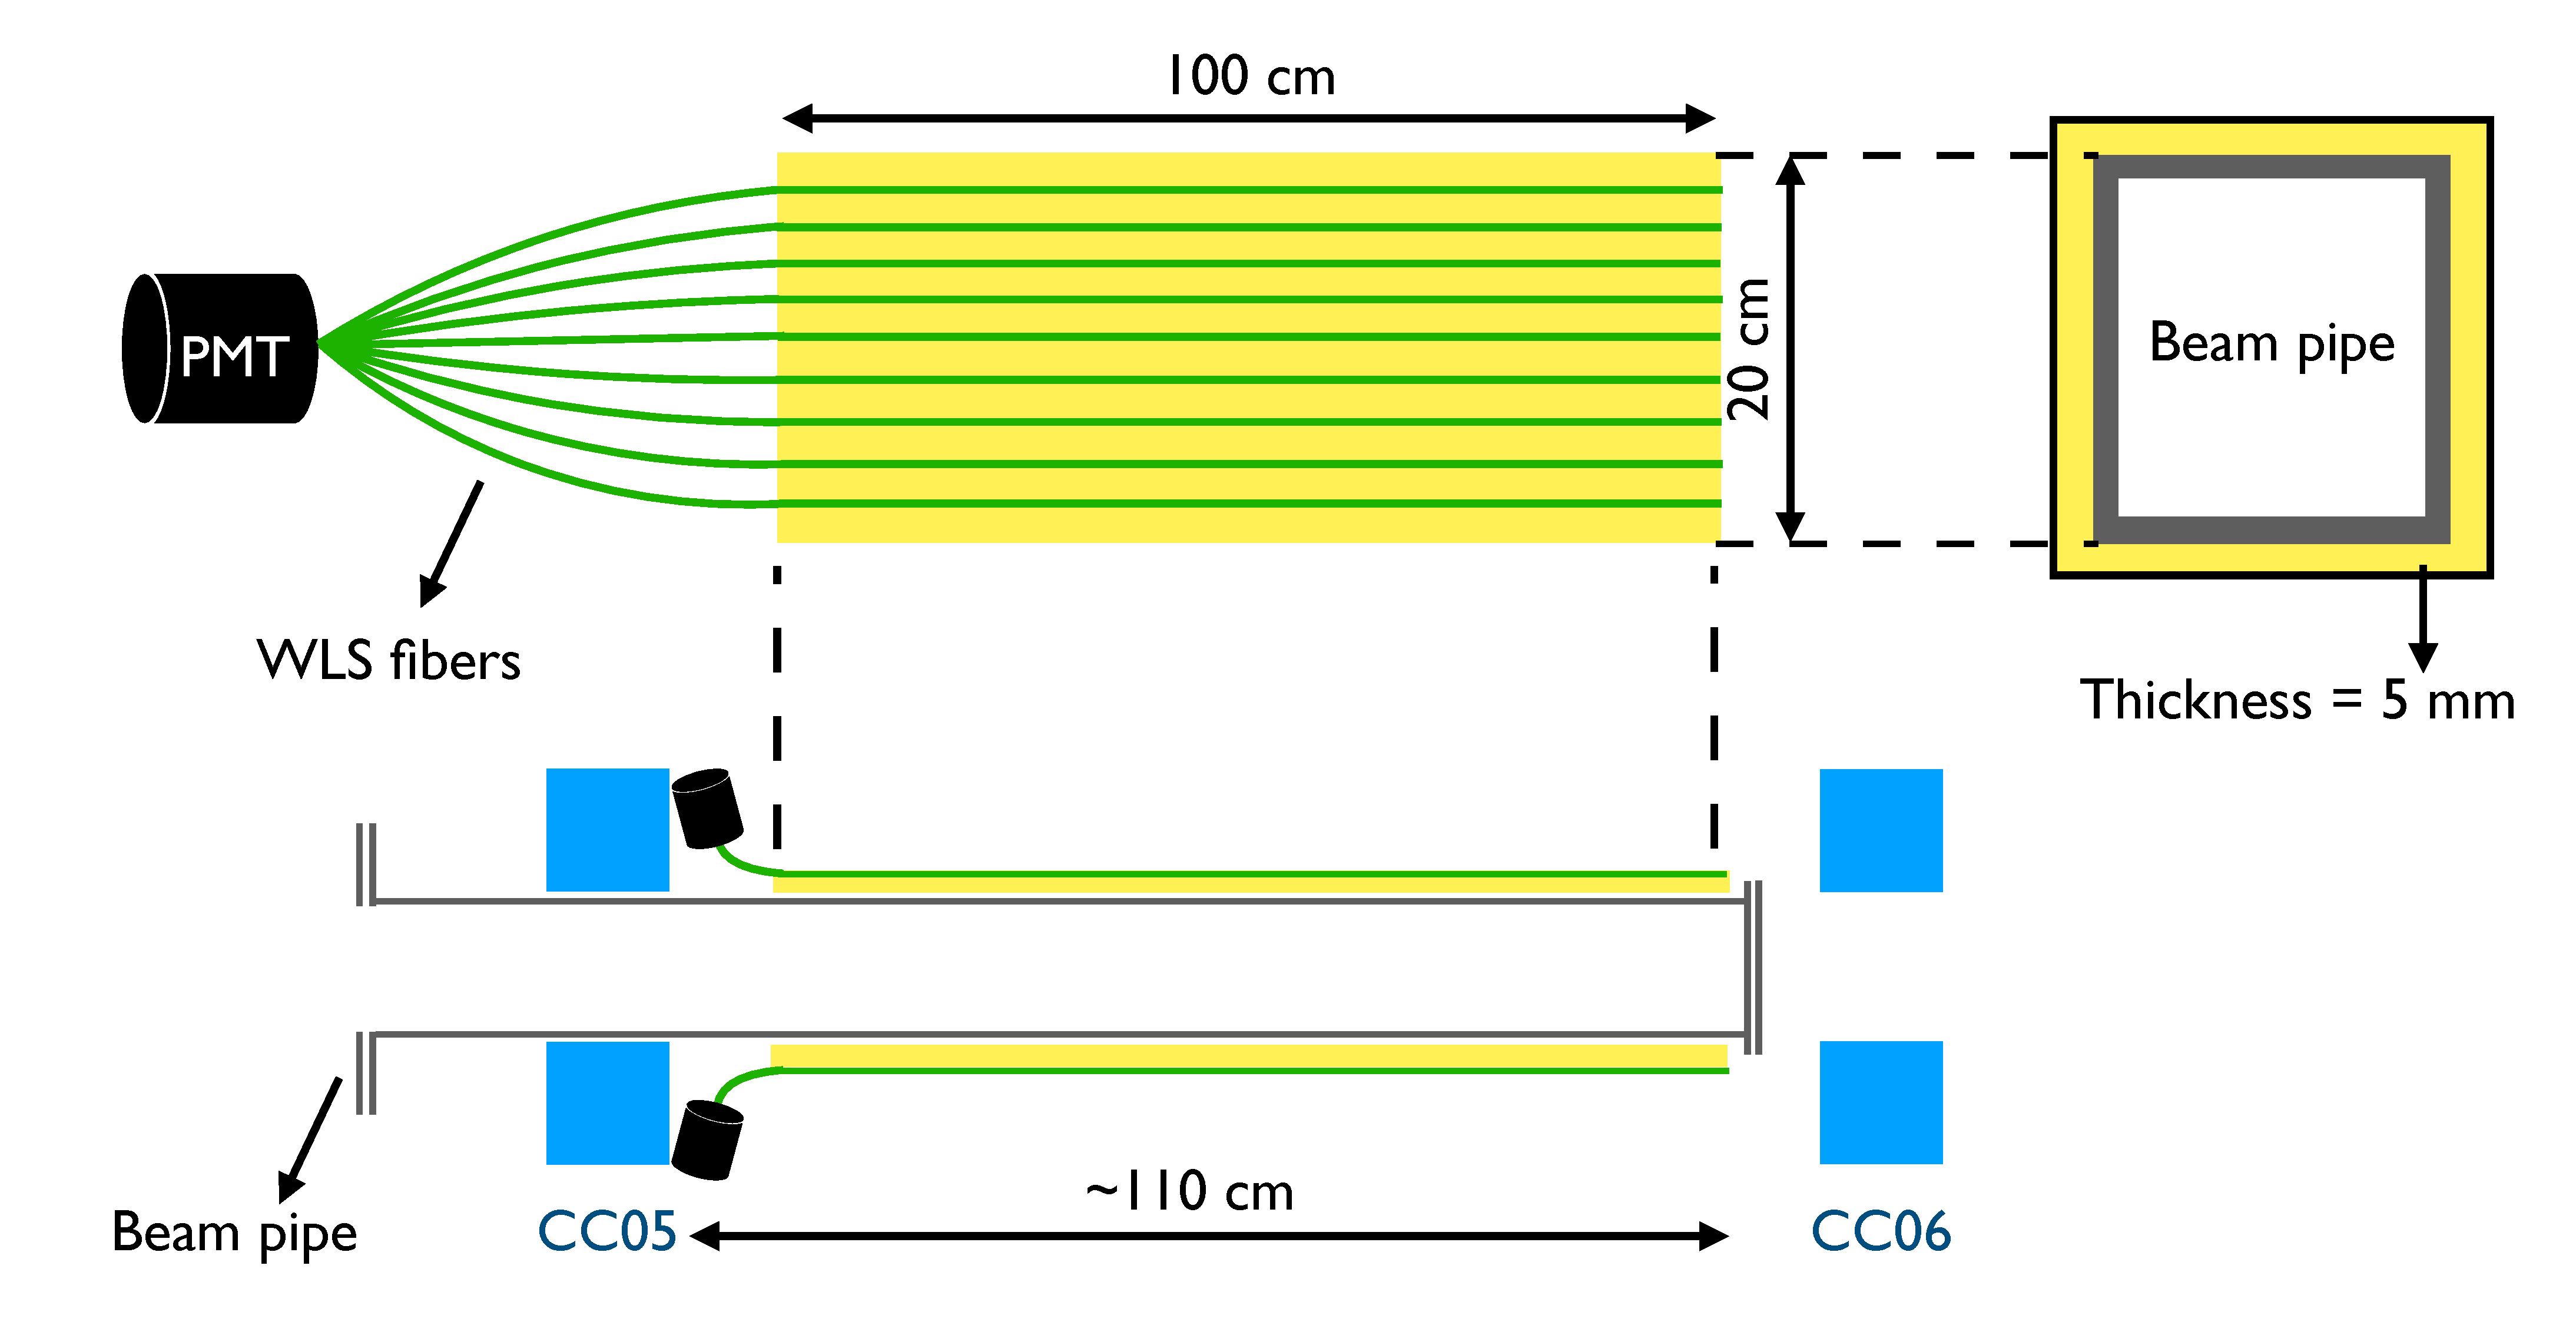
\includegraphics[width=0.9\textwidth]{Figures/Chapter3/BPCV.pdf}
\caption{A schematic diagram of BPCV \parencite{BPCV}.}
\label{fig:BPCV}
\end{center}
\end{figure}

%
%% 3-10 Beam hole counters
%%%%%%%%%%%%%%%%%%%%%%%%%%%
\subsection{Beam Hole Veto Counters}
\label{sec:beam_hole_counter}
The in-beam veto counters are located at the end of the KOTO detector, which are regarded as the last-ditch attempt to capture the extra particles in a $K_L^0$ decay traveling along the beam. These counters typically suffer from the numerous neutrons in the beam and needs to tolerate the high-rate environment. As a result, the balance between the neutron insensitivity and the detection power of the escaping particles is a crucial topic for designing beam hole counters.

\subsubsection{Charge veto at beam hole}
The Beam Hole Charge Veto (BHCV) counter \parencite{BHCV, BHCV2}, a multi-wire chamber filled with mixed gas of Tetrafluoromethane (CF4) and n-Pentane, is primarily constructed at the beam region to detect $\pi^{\pm}$s in the ${K_L^0 \to \pi^+ \pi^- \pi^0}$ decay. Figure~\ref{fig:BHCV} describes the principle of BHCV. When a charged particle passes through the chamber, the surrounding gas is ionized into ions and electrons. Under the influence of the electric field, the resulting charges are collected through the wires and cause the pulses. 

BHCV features the thin gap between the wires and the planes, which enable the rapid response to the gaseous ionization. Moreover, the light materials are utilized to eliminate the interactions with the neutrons and the photons contained in the beam. BHCV has three modules in a row along the beam. The coincident signals in more than two consecutive modules are required to reduce the noise.

\begin{figure}[h]
\begin{center}
\captionsetup{width=.99\linewidth}
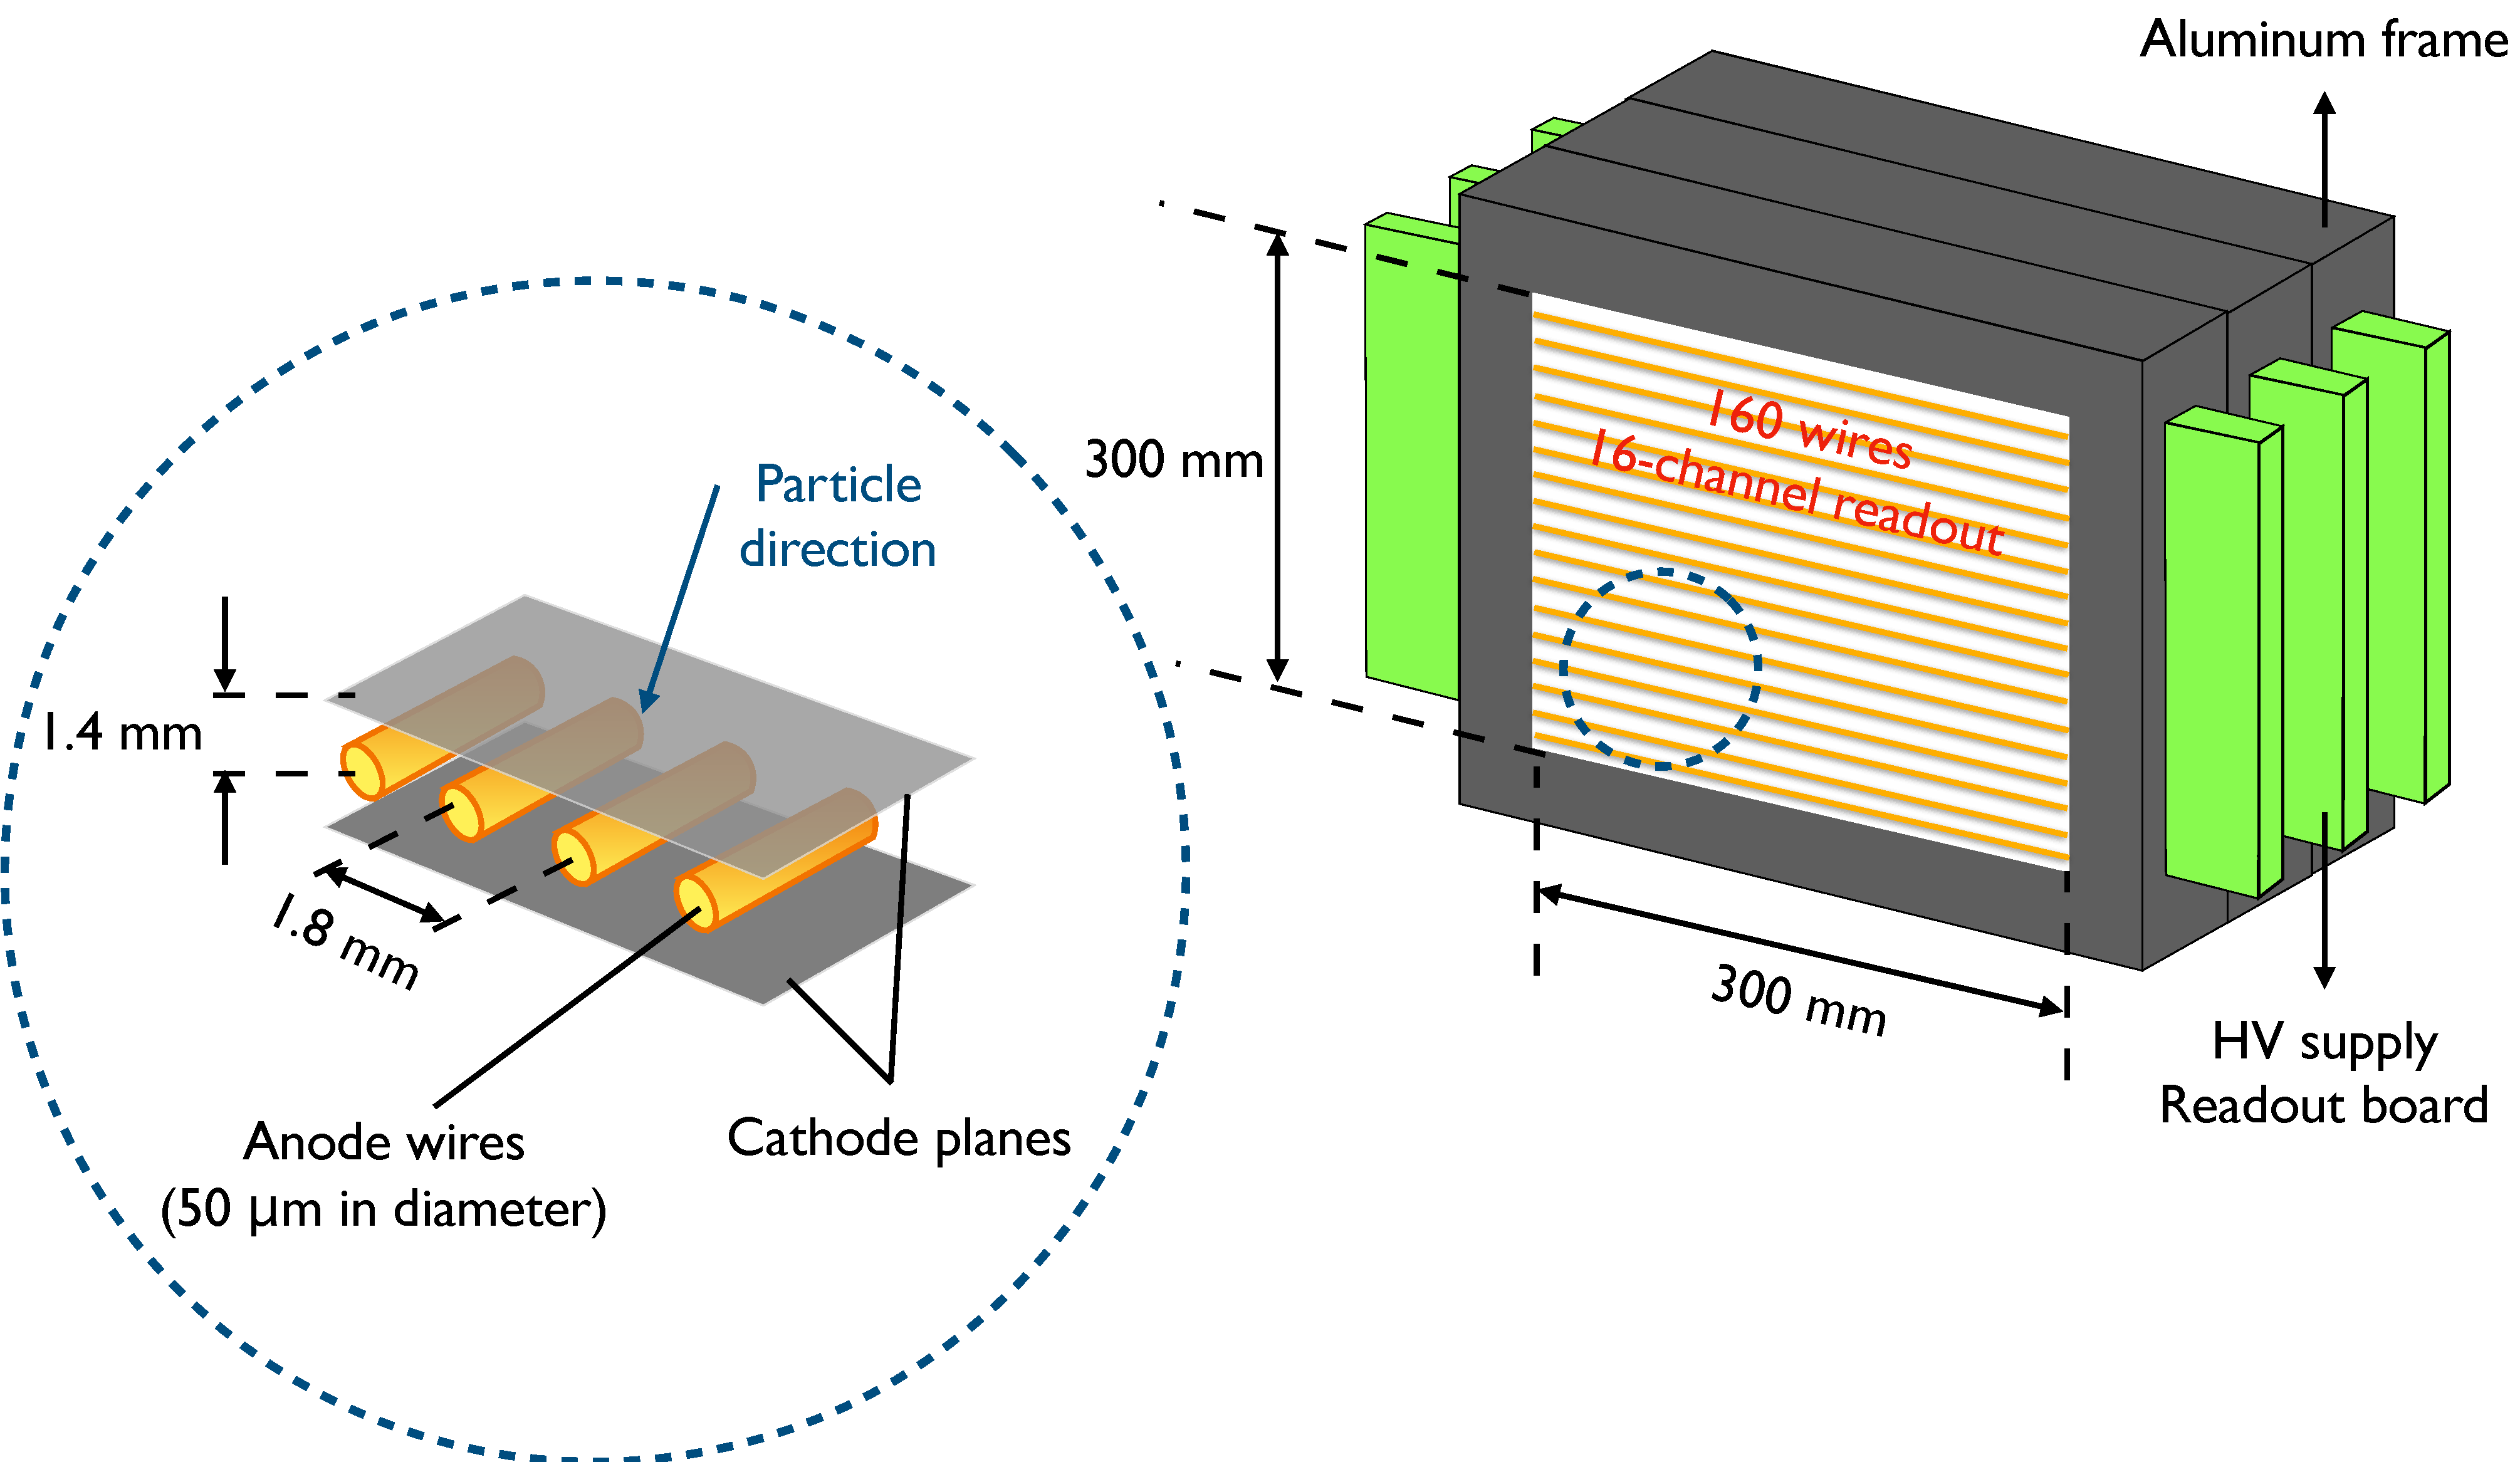
\includegraphics[width=0.99\textwidth]{Figures/Chapter3/BHCV.pdf}
\caption{A schematic diagram of BHCV \parencite{BHCV}.}
\label{fig:BHCV}
\end{center}
\end{figure}


%\begin{figure}[h]
%\begin{center}
%\captionsetup{width=.99\linewidth}
%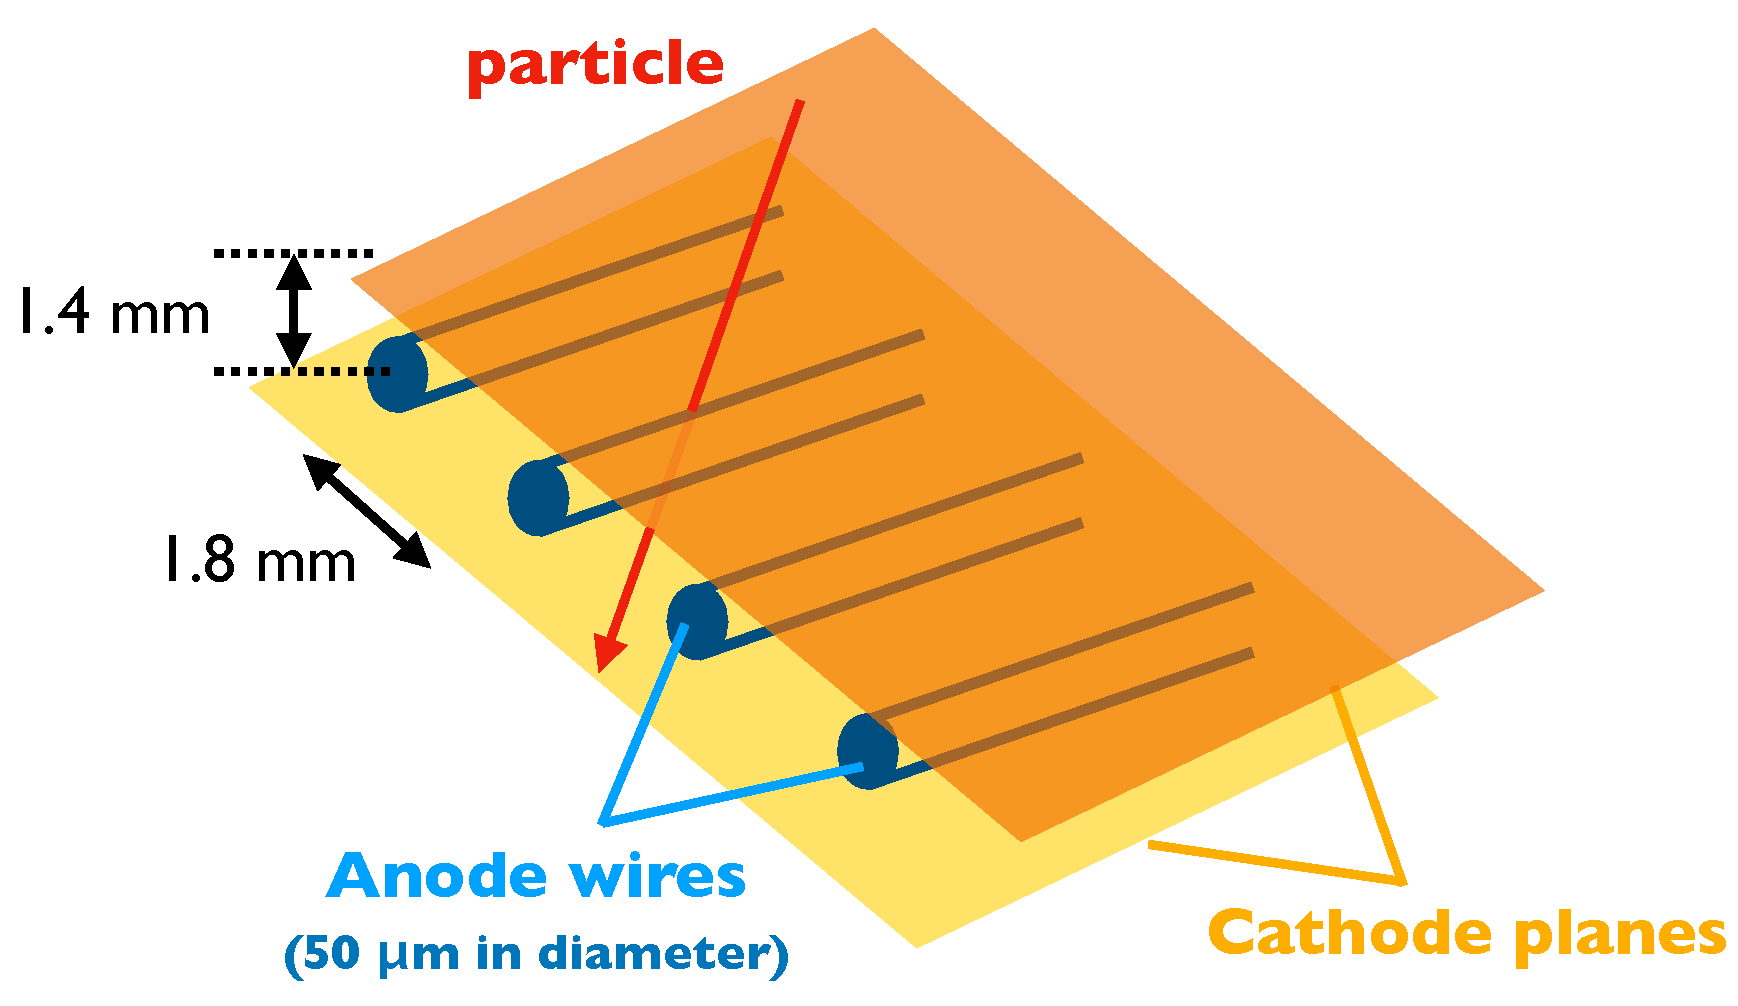
\includegraphics[width=0.7\textwidth]{Figures/Chapter3/BHCV_schematic.pdf}
%\caption{Principle of a ulti-wire chamber for BHCV.}
%\label{fig:BHCV_schematic}
%\end{center}
%\end{figure}


%\begin{figure}[h]
%\begin{center}
%\captionsetup{width=.99\linewidth}
%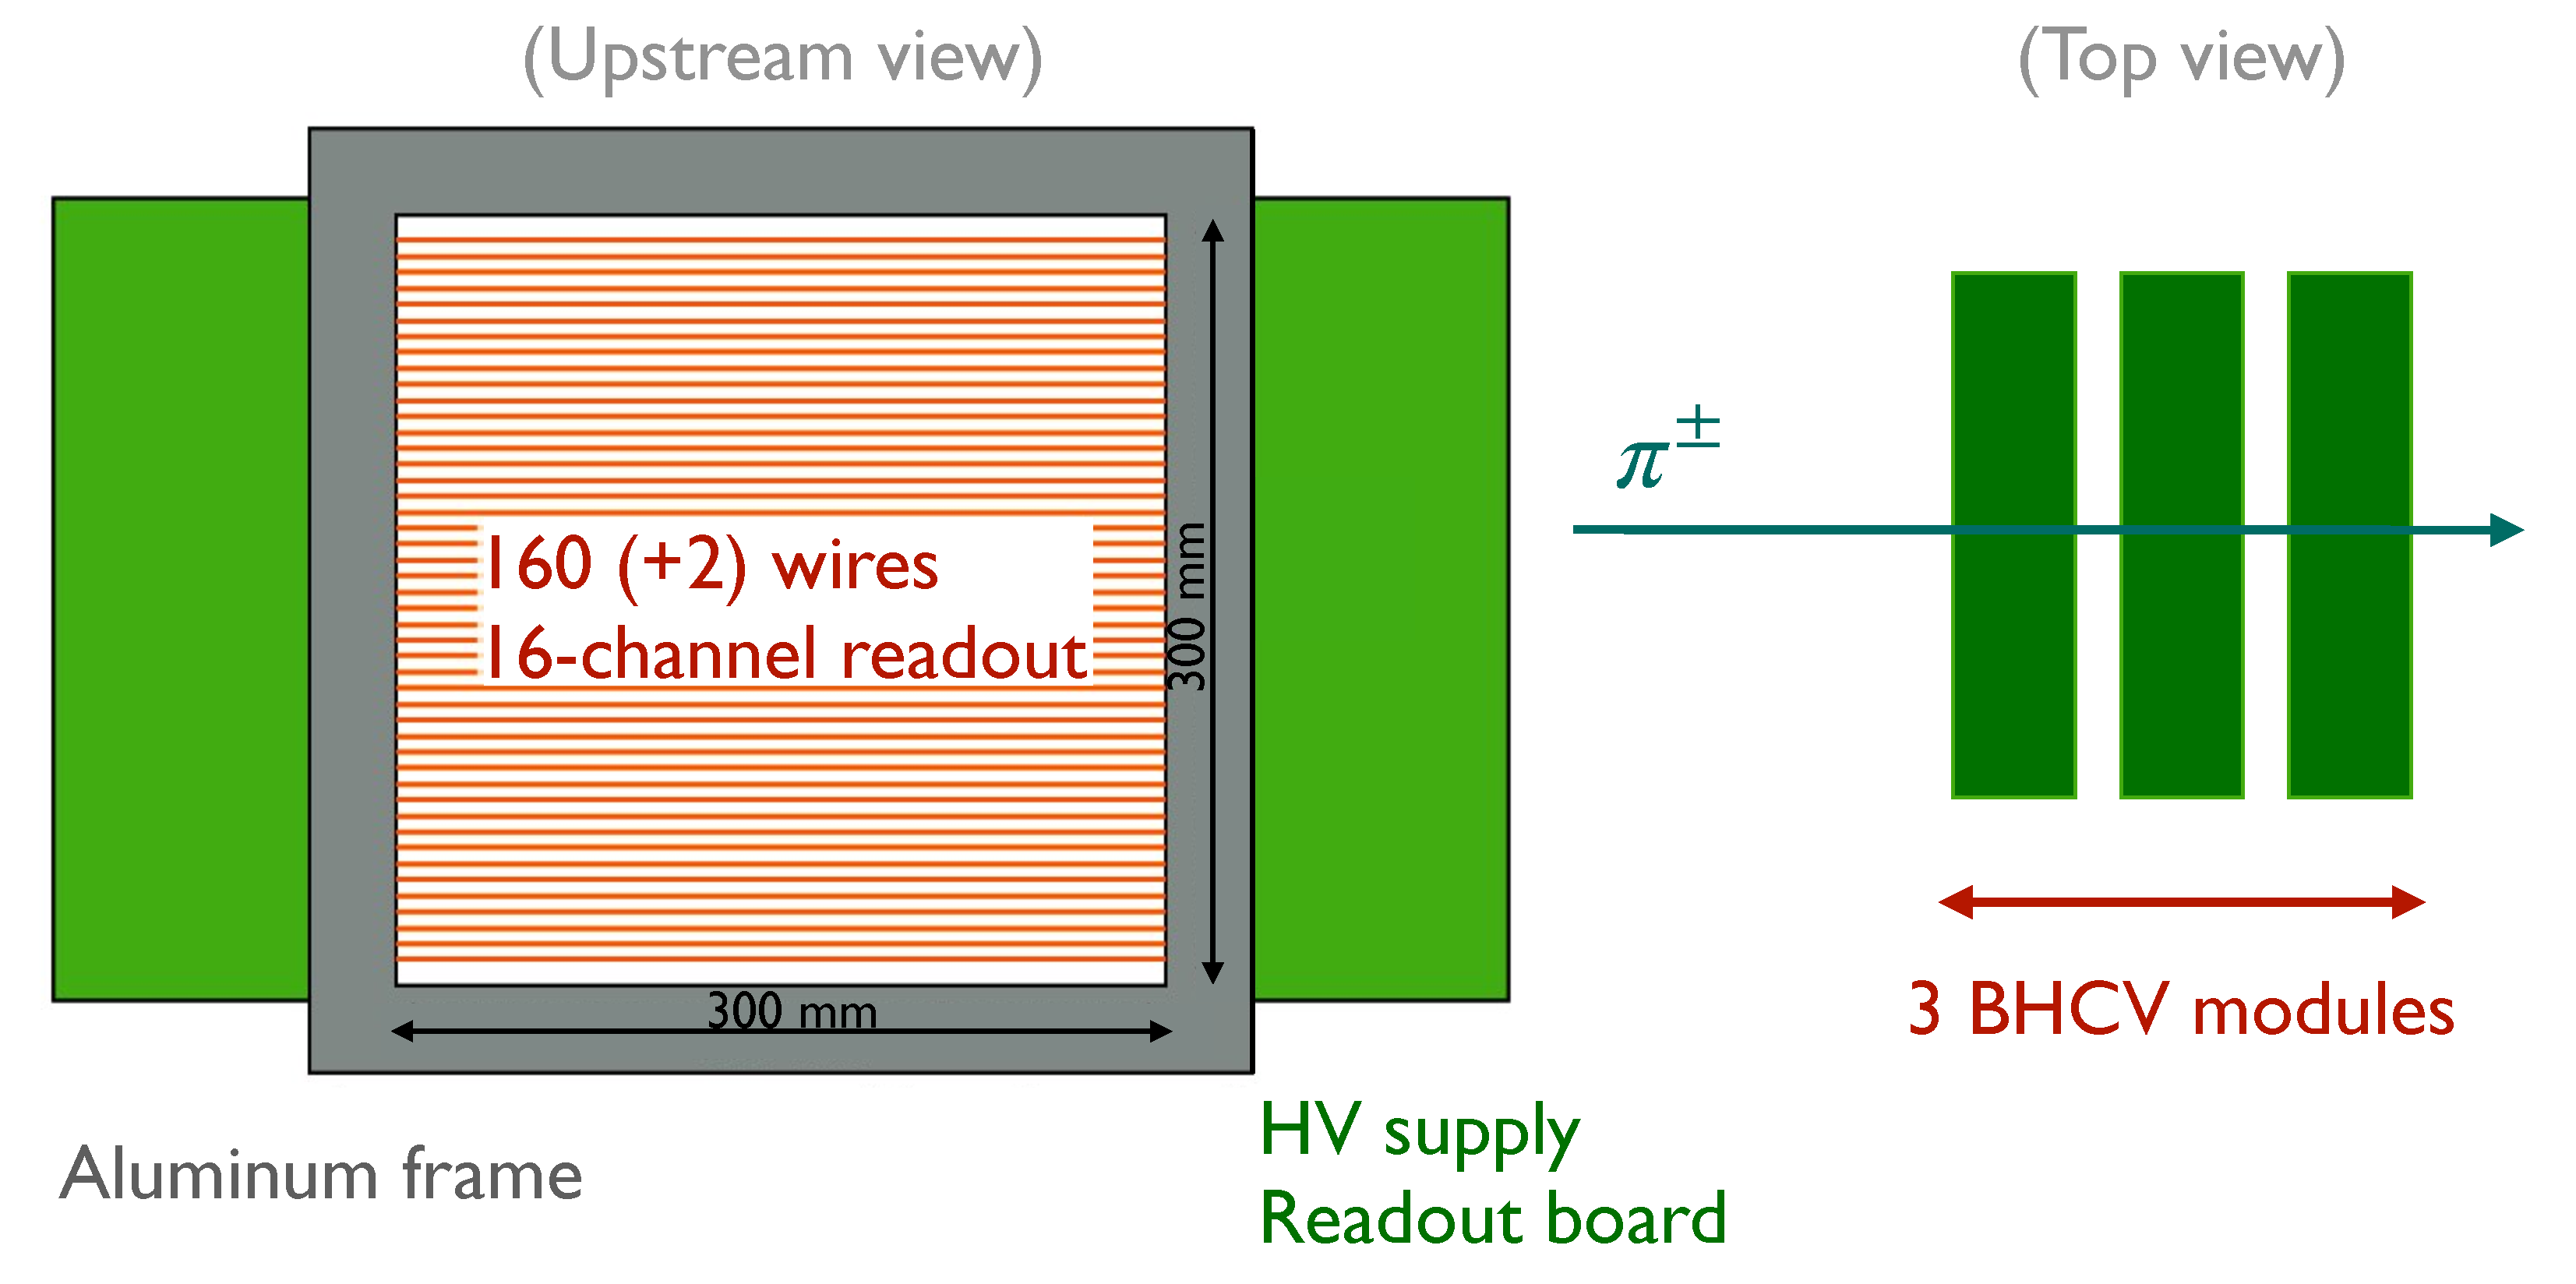
\includegraphics[width=0.8\textwidth]{Figures/Chapter3/BHCV_config.pdf}
%\caption{A graphical illustration of BHCV (Figure courtesy of \parencite{BHCV} with modifications).}
%\label{fig:BHCV_config}
%\end{center}
%\end{figure}

\subsubsection{Photon veto at beam hole}
If one of the photons in a $\pi^0\to2\gamma$ decay is too soft, the other tends to boost forward and escape into the beam hole. Because soft photons are barely detectable, the sensitivity to the energetic photons in the beam translates into the background level, especially for the ${K_L^0 \to \pi^0 \pi^0}$ background. The two subdetectors, Beam Hole Photon Veto (BHPV) \parencite{BHPV} and Beam Hole Guard Counter (BHGC) \parencite{BHGC}, are \v{C}erenkov counters for photon veto. As Figure \ref{fig:BHPV_BHGC} shows, an energetic photon strikes a lead converter and produces an electron-positron pair. The \v{C}erenkov light is then radiated by the material (an aerogel tile for BHPV or an acrylic plate for BHGC), guided to either side of the module, and collected by a PMT.  In contrast, a \v{C}erenkov light is scarcely produced by slow-neutrons because the generated charged particle tends to be slower than the speed of light in the material.

BHPV is the in-beam counter that consists of 16 modules in a row and BHGC is the beam-edge counter to complement the photon detection. A concrete shield is implemented in front of BHPV to eliminate the shower splashing back to its upstream counters. Both BHPV and BHGC possess an approach to further suppress the fake signals due to the \v{C}erenkov light induced by slow neutrons. BHPV requires the coincident signals in consecutive modules, because the electromagnetic shower developed by energetic photons tends to spread forward, while the secondary particles from slow-neutron interactions tend to propagate isotropically. BHGC inhibits the \v{C}erenkov light transmitting along the plate if the resulting angle is smaller than the critical angle.

%\begin{figure}[h]
%\begin{center}
%\captionsetup{width=.99\linewidth}
%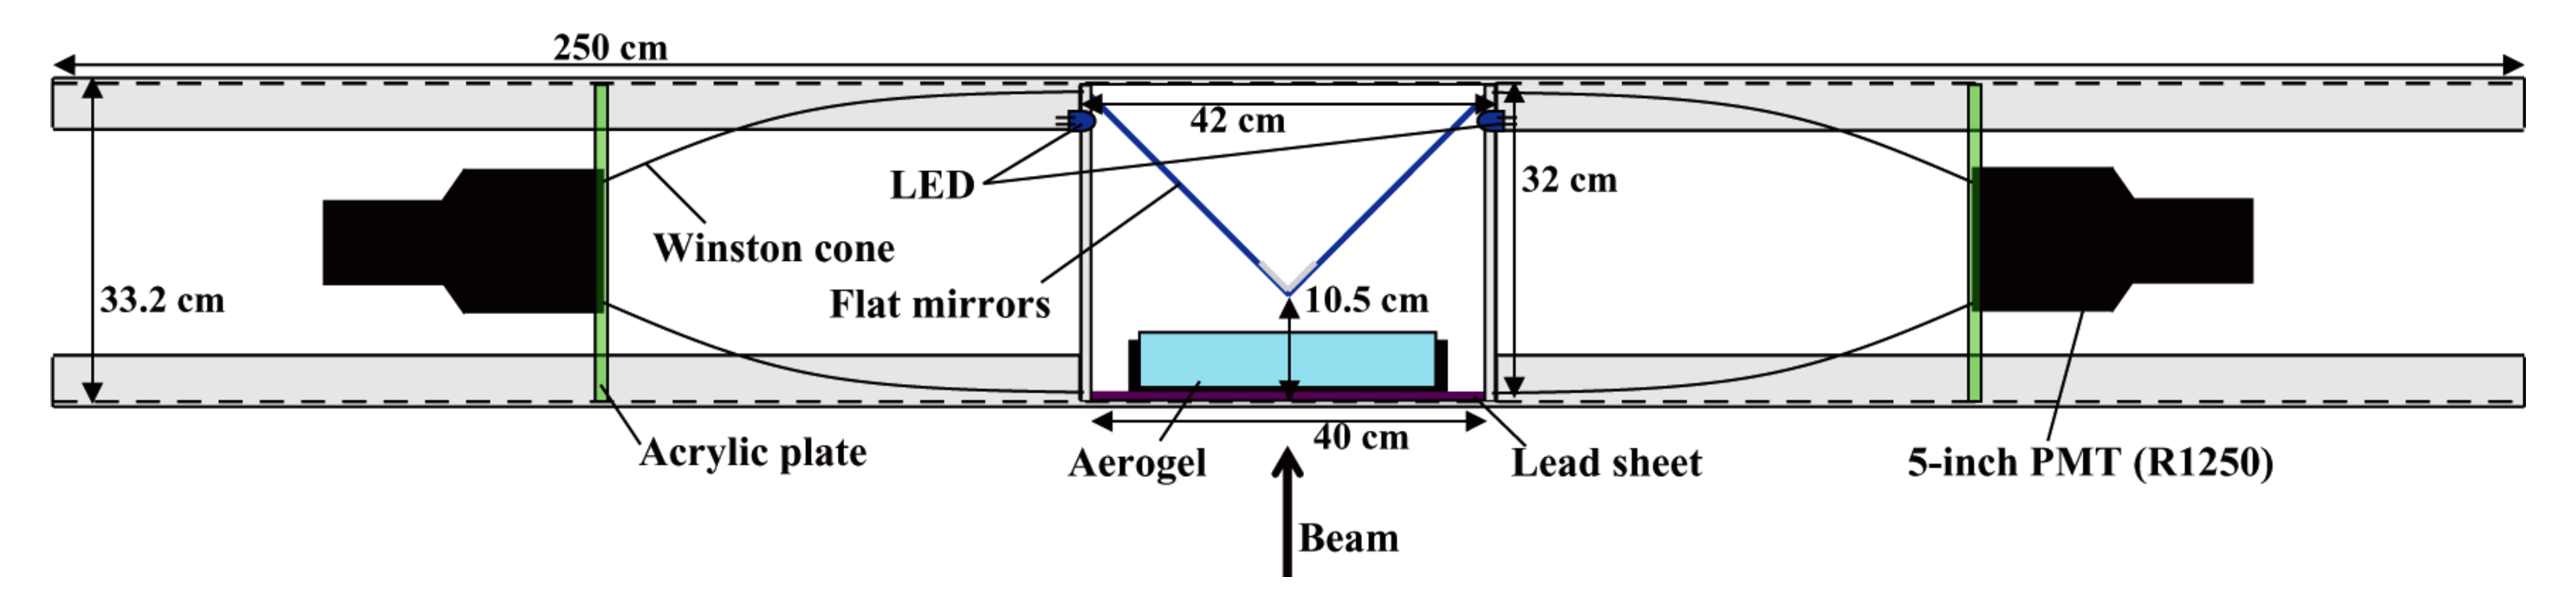
\includegraphics[width=0.9\textwidth]{Figures/Chapter3/BHPV_module.pdf}
%\caption{A schematic diagram of a BHPV module (Figure courtesy of \parencite{BHPV}).}
%\label{fig:BHPV_module}
%\end{center}
%\end{figure}

%\begin{figure}[h]
%\begin{center}
%\captionsetup{width=.99\linewidth}
%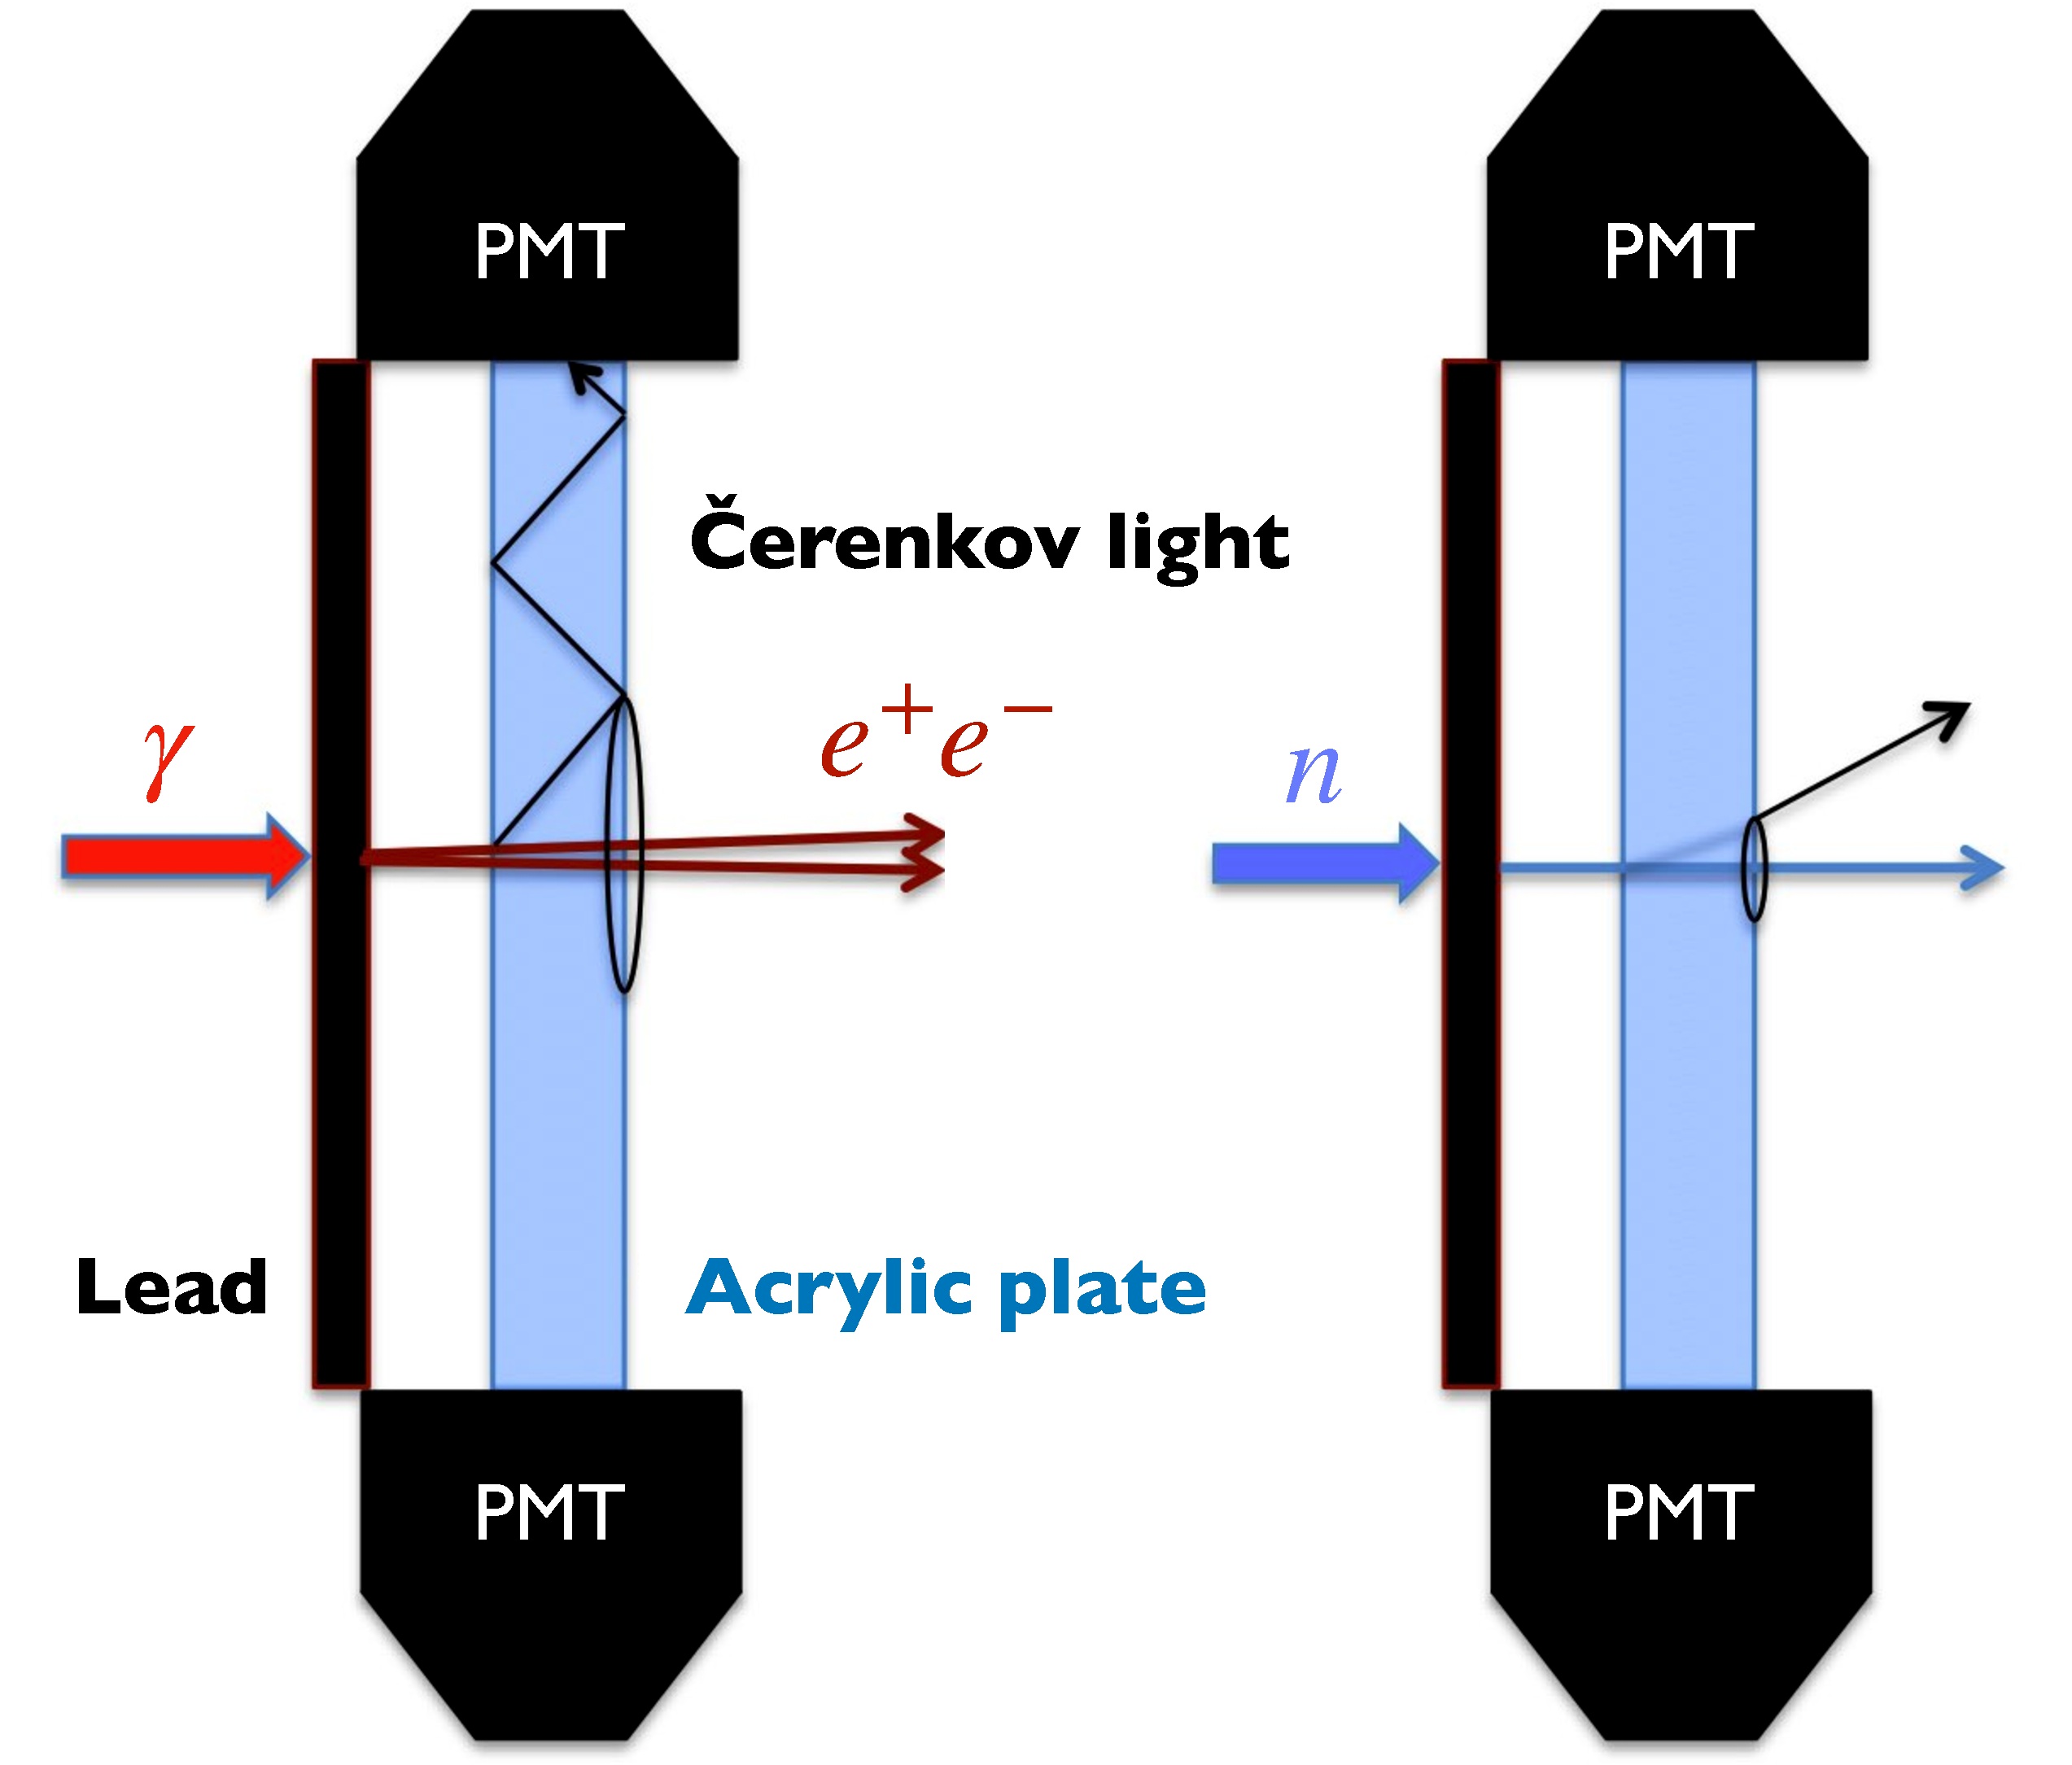
\includegraphics[width=0.5\textwidth]{Figures/Chapter3/BHGC_principle.pdf}
%\caption{Particle responses at BHGC (Figure courtesy of \parencite{BHGC2}).}
%\label{fig:BHGC_principle}
%\end{center}
%\end{figure}

%BHPV is the in-beam counter that consists of 16 modules in a row and BHGC is the beam-edge counter to complement the photon detection, as shown in Figure \ref{fig:BHPV_BHGC}. A concrete shield is implemented in front of BHPV to eliminate the shower splashing back to its upstream counters.

%\begin{figure}[h]
%\begin{center}
%\captionsetup{width=.99\linewidth}
%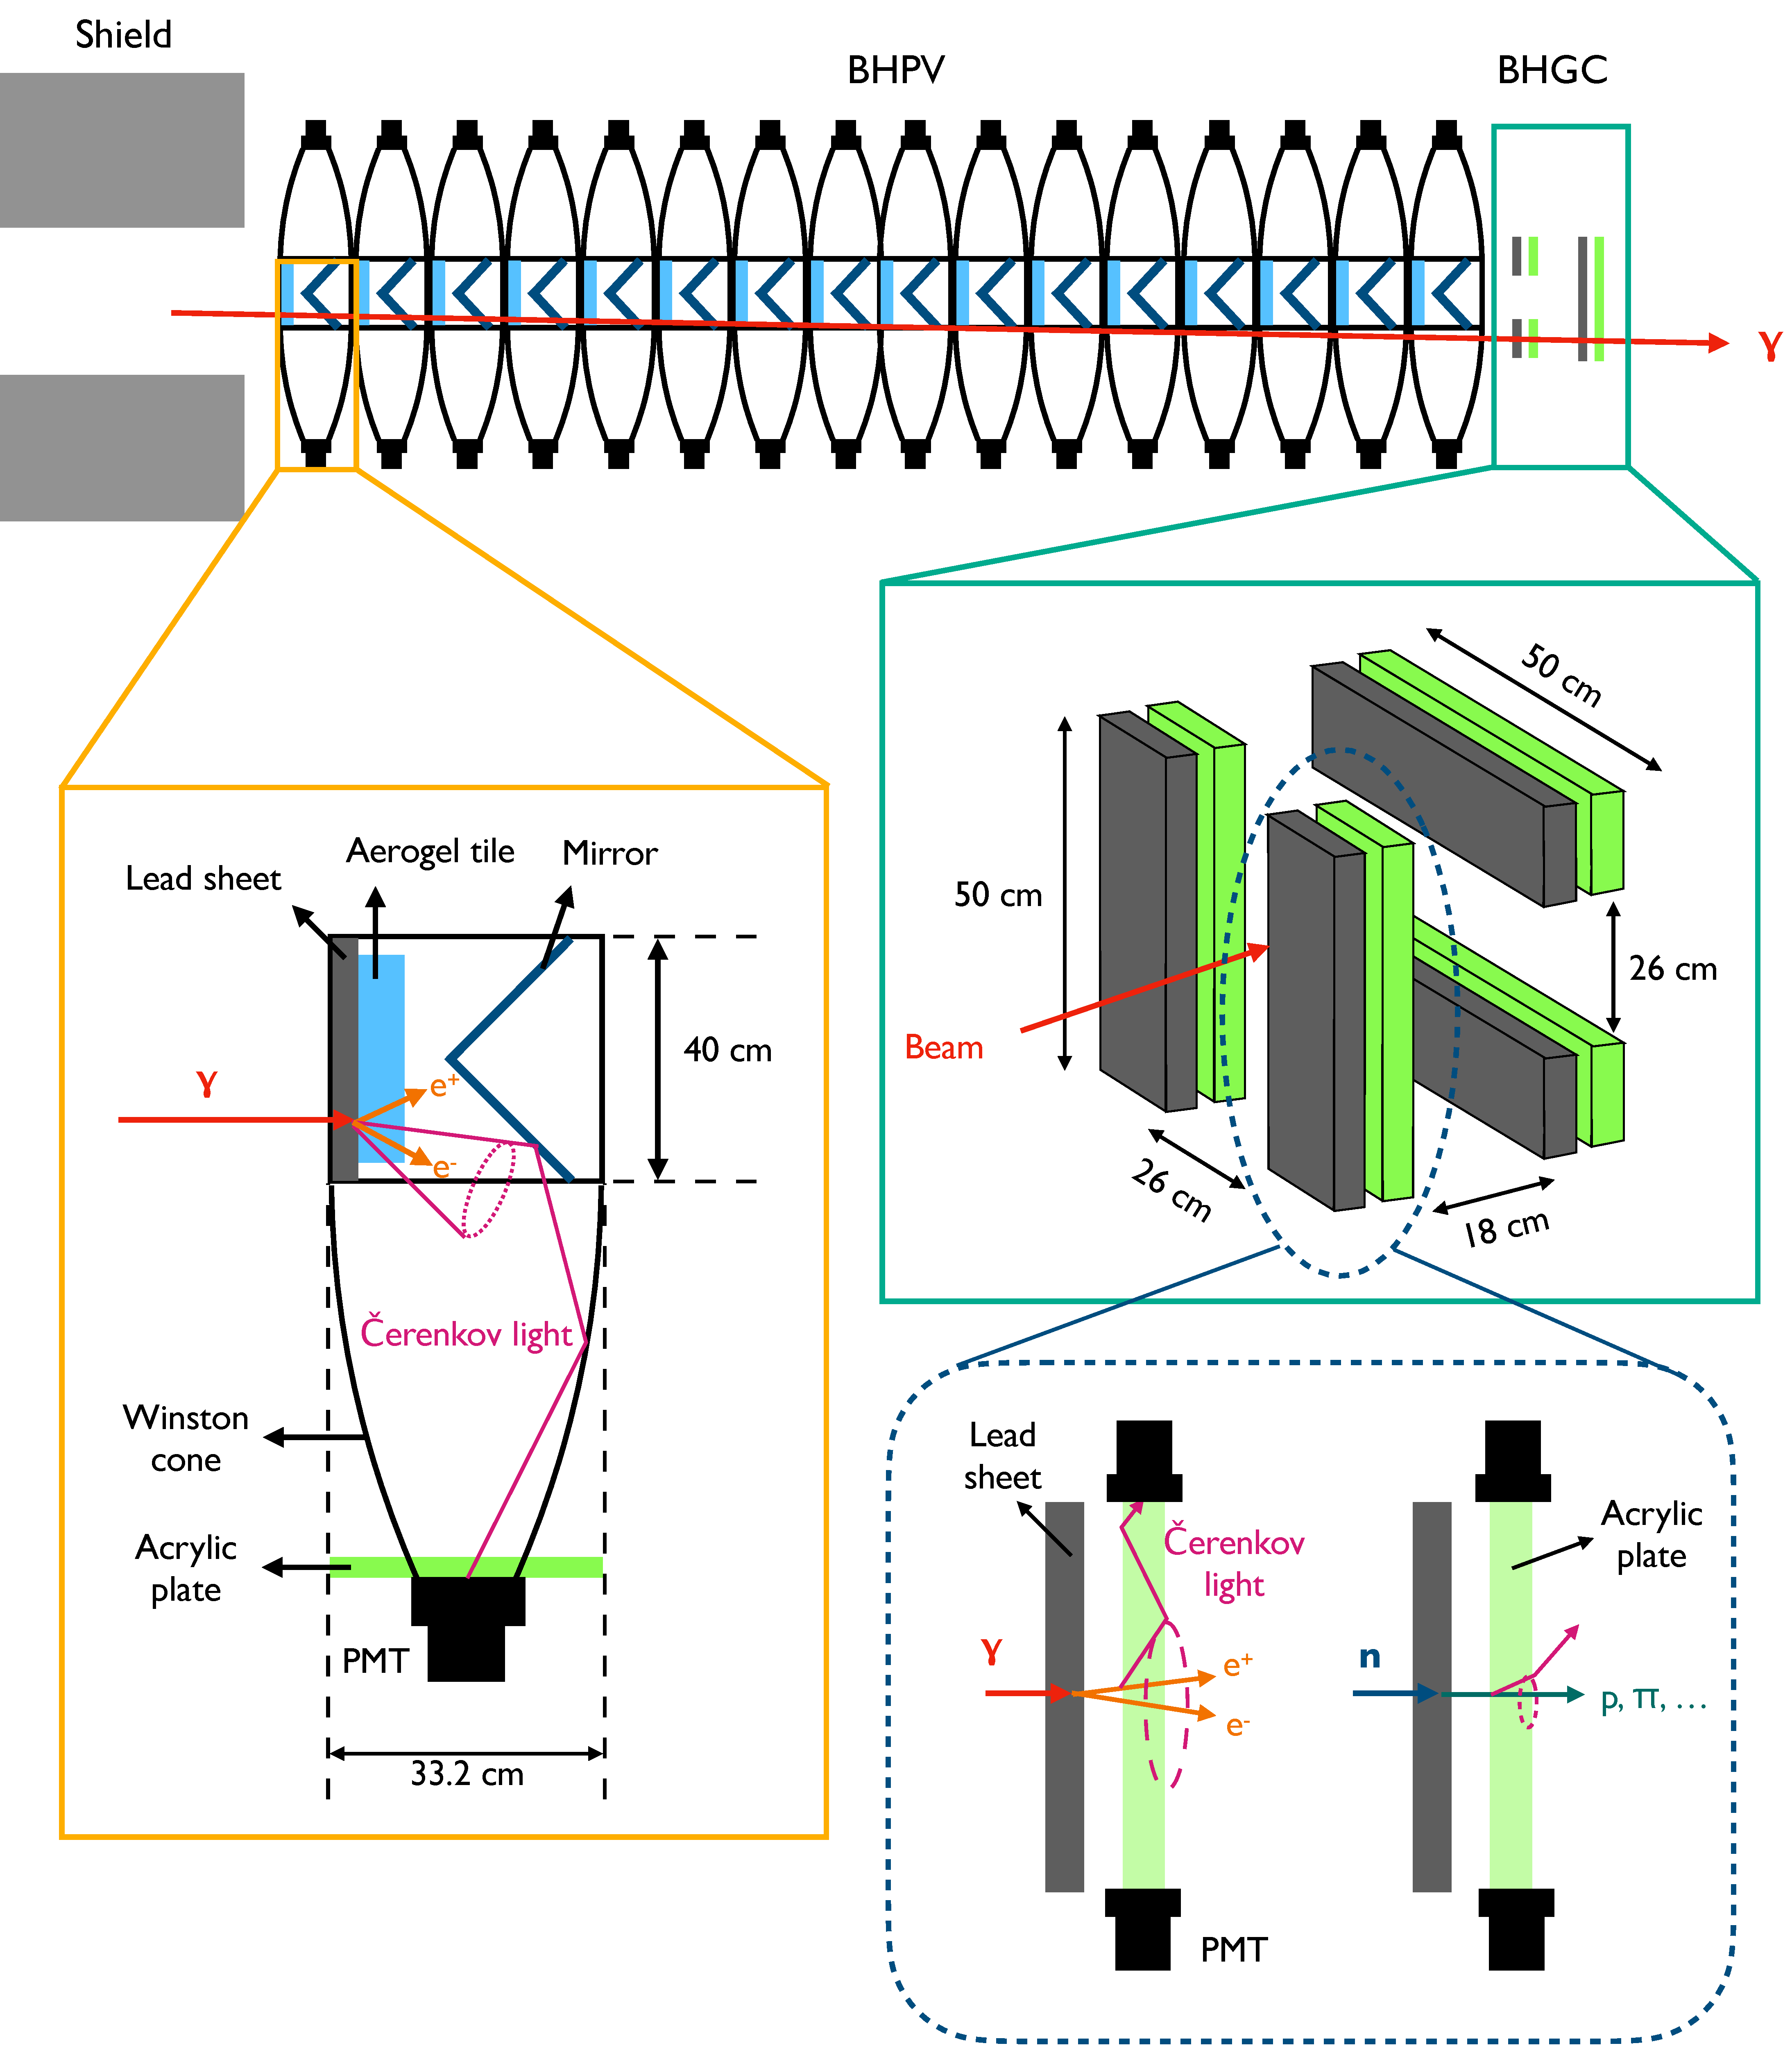
\includegraphics[width=0.9\textwidth]{Figures/Chapter3/BHPV_BHGC.pdf}
%\caption{A graphical illustration of BHPV and BHGC. (Figure courtesy of \parencite{BHPV} with modifications).}
%\label{fig:BHPV_BHGC}
%\end{center}
%\end{figure}

\begin{figure}[h]
\begin{center}
\captionsetup{width=.99\linewidth}
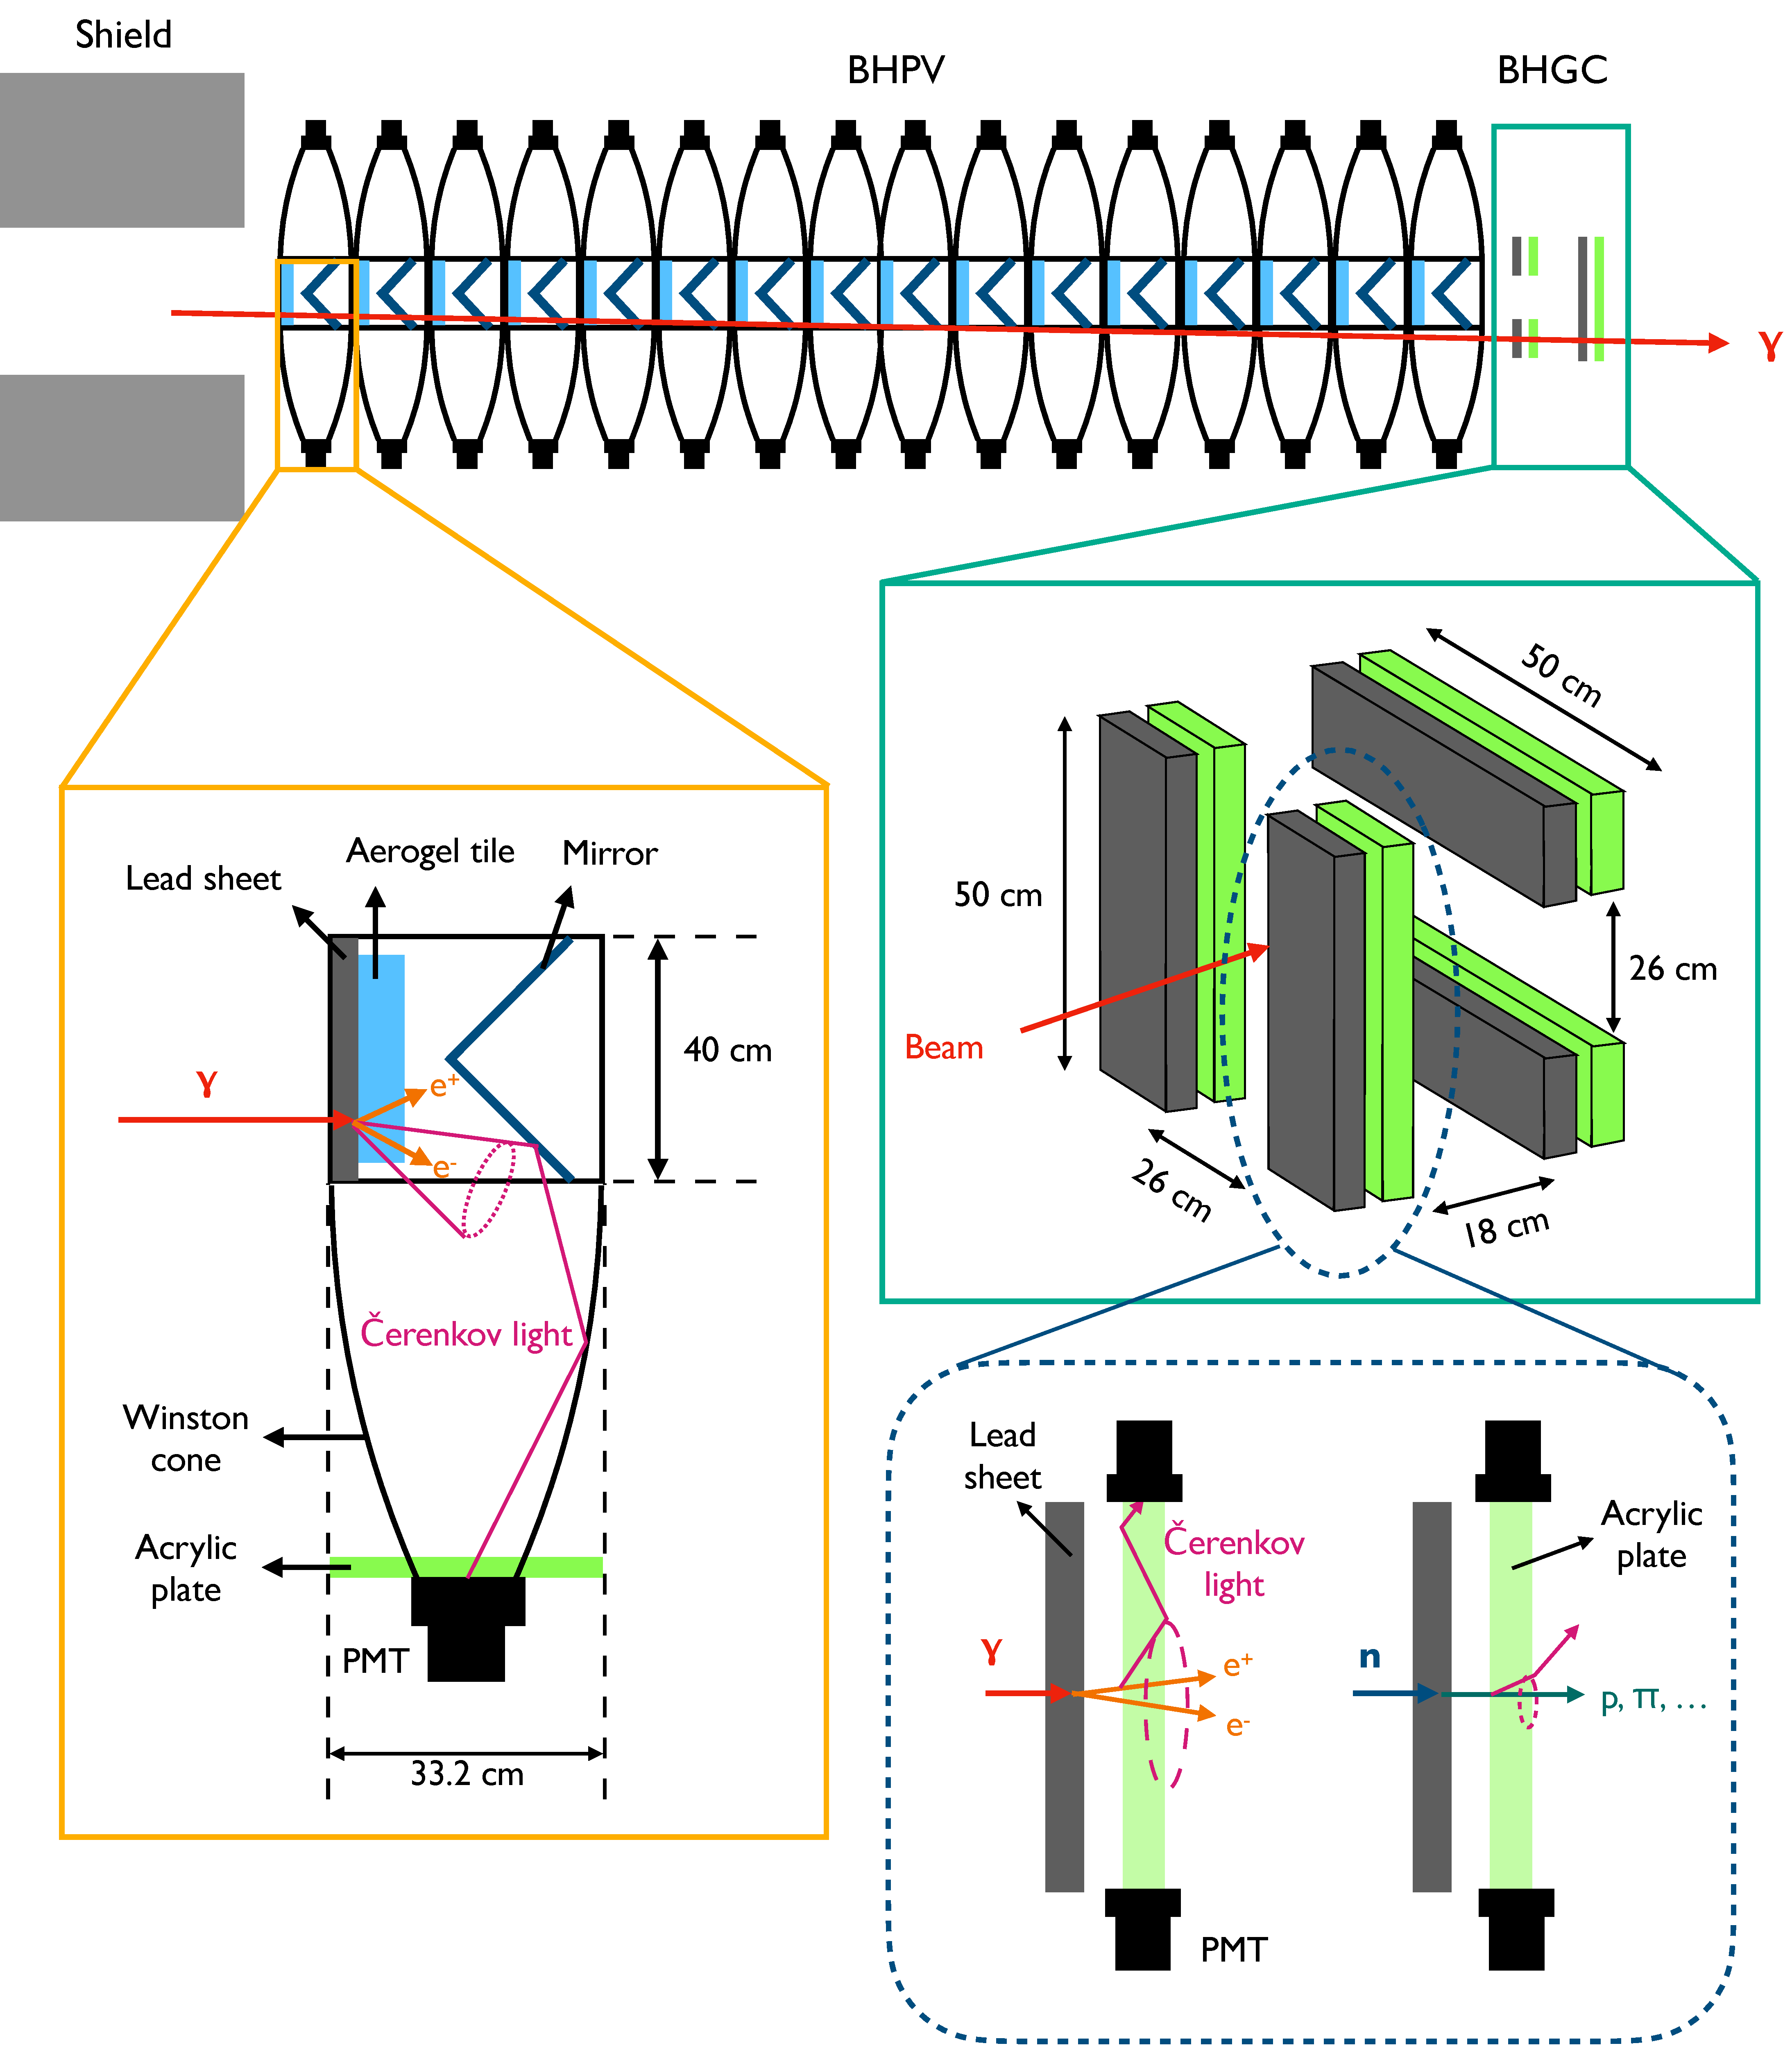
\includegraphics[width=0.99\textwidth]{Figures/Chapter3/BHPV_BHGC.pdf}
\caption{A schematic diagram of BHPV and BHGC \parencite{BHPV, BHGC}.}
\label{fig:BHPV_BHGC}
\end{center}
\end{figure}

